\documentclass[10pt]{article}
\usepackage{packages}

\title{\huge{Relazione laboratorio di complementi di inorganica}
\vspace{1mm}\\
\Large{Anno Accedemico 2022/2023}}
\author{\href{mailto:m.fiaschi10@studenti.unipi.it}{Fiaschi Matteo\footnote{Materiale aggiuntivo si può trovare nella seguente reporsitory sul mio account \href{https://github.com/mfiaschi5/labinorganica}{GitHub}.}} \and \href{mailto:a.ariosto@studenti.unipi.it}{Alberto Ariosto}}
\date{31 maggio 2023}



\begin{document}
\maketitle
\begin{center}
    \textbf{Abstract}
\end{center}
\noindent \textit{ In questo documento sono riportate le procedure sperimentali, le osservazioni e dati raccolti durante il Laboratorio di Complementi di Chimica Inorganica. Sono state svolte le sintesi di alcuni complessi di nichel con rispettive caratterizzazioni tramite misure magnetiche e spettrometria Uv-Vis. Sintesi del cobalto salen e cobalto(II) acetato in atmosfera inerte, con caratterizzazione del primo tramite assorbimento dell'ossigeno atmosferico in DMSO e spettro IR e del secondo con H-NMR in cloroformio deuterato. Preparazione del complesso cobalto dinosar, purificazione tramite cristallizzazione e  caratterizzazione tramite spettro H-NMR in acqua deuterata. Sintesi dell'idruro di  cobalto e assorbimento e desorbimento termico di idrogeno su ossido di tungsteno con relativo test di conducibilità. }




\section{Preparazione e misure magnetiche per complessi di \ce{Ni(II)}}

\subsection{Preparazione di \ce{Ni(en)3Cl2.2H2O} }
\begin{figure}[ht!]
    \centering
    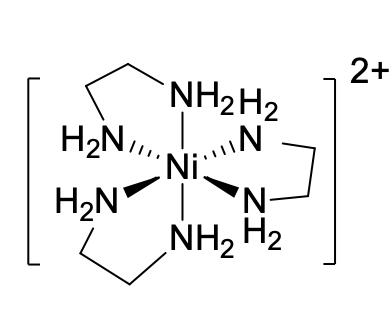
\includegraphics[width=0.3\linewidth]{foto/nien.png}
    \caption{Complesso \ce{Ni(en)3Cl2} }
    \label{fig:nien}
\end{figure}
\subsubsection{Procedura sperimentale}
Abbiamo pesato alla bilancia tecnica $3.00 \mathrm{~g}$ di $\mathrm{NiCl}_2 \cdot 6 \mathrm{H}_2 \mathrm{O}$\footnote{ E' stato utilizzato il nichel cloruro anidro, la massa pesata quindi differisce dal valore prestabilito dalle dispense. Nella sezione dedicata ai calcoli si utilizza la massa aggiustata per il sale anidro} e li abbiamo disciolti in un becher con $1.5 \mathrm{~mL}$ d'acqua sotto agitazione e con l'aiuto di un debole riscaldamento. Nello stesso recipiente abbiamo aggiunto $2.8 \mathrm{~mL}$ di etilendiammina e immerso il tutto in un bagno di ghiaccio. Si osserva la precipitazione di un complesso viola. In seguito abbiamo addizionato tramite cilindro graduato $7.5 \mathrm{~mL}$ di etanolo freddo per favorire la cristallizzazione. Quindi abbiamo filtrato su Buchner e lavato con due aliquote da $5.0 \mathrm{~mL}$ di etanolo. Infine, dopo aver asciugato sul Buchner i cristalli, li abbiamo trasferiti in una provetta precedentemente pesata alla bilancia analitica per essere seccati sottovuoto alla pompa meccanica.
\subsubsection{Commenti e osservazioni}
La dissoluzione del solido è stata difficoltosa, abbiamo dovuto scaldare e far scorrere l'ancoretta su tutto il fondo del becher per diversi minuti. Questo può essere dovuto alla granulometria del nichel che si era \textit{cementificato} formando degli agglomerati duri, difficili da rompere tramite agitazione magnetica. Alcune possibili soluzioni a questo problema possono essere: evitare questi granuli durante la pesata, pestellare il solido per omogenizzarlo ( questo può essere eseguito nel becher con una bacchetta di vetro oppure in un mortaio, in quest'ultimo caso l'operazione va eseguita prima della pesata in quanto altrimenti avremo che parte del solido rimarrebbe attaccata alle pareti del pestello e del mortaio).
Abbiamo notato inoltre la variazione di colore non è stata diretta ma è passata per colorazioni intermedie. Questo fenomeno può essere spiegato dal fatto che la completa complessazione procede per specie intermedie come \ce{[Ni(en)(OH2)4]^{2+} }, \ce{[Ni(en)2(OH2)2]^{2+} }. \footnote{Si presume che ulteriori intermedi come \ce{[Ni(en)(OH2)5]^{2+} } e  \ce{[Ni(en)2(OH2)3]^{2+} } si convertano abbastanza velocemente da provocare transizioni di colore visibili della soluzione   }


\subsubsection{Calcoli e analisi dei dati}

Il numero di moli di $\mathrm{NiCl}_2 \cdot 6 \mathrm{H}_2 \mathrm{O}$ che occorrono sono
$$
n_{\mathrm{NiCl}_2}=\frac{3.00 \mathrm{~g}}{237.70 \mathrm{~g} / \mathrm{mol}}=0.0126 \mathrm{~mol}
$$
che convertite in massa di \ce{NiCl2} anidro da pesare si trasformano in

\[  {m_{\ce{NiCl2}}} = n_{\mathrm{NiCl}_2} \cdot {M_{\ce{NiCl2}}} = 0.0126 \mathrm{~mol} \cdot 129.6  \ \text{g/mol} = 1.63 \text{g} \]
Per l'etilendiammina
$$
n_{\mathrm{en}}=\frac{2.8 \mathrm{~mL} \cdot 0.899 \mathrm{~g} / \mathrm{mL}}{237.7 \mathrm{~g} / \mathrm{mol}}=0.0419 \mathrm{~mol}
$$
Notiamo che l'etilendiammina è in eccesso, infatti il rapporto $\frac{n_{\text{en}}}{{n_{\ce{NiCl2}}}} = 3.33 > 3$
Di conseguenza, poiché l'etilendiammina è più che stechiometrica, deduciamo che il reagente limitante è il sale di nichel. 

La resa sarà dunque calcolata basandosi sul nichel iniziale\footnote{Un eccesso di etilendiammina è necessario per garantire la completa complessazione del nichel a tris(etilendiammina)nichel dicloruro. Questo non inficerà la purezza del prodotto in quanto l'eccesso sarà rimosso dai lavaggi con etanolo}. 
La massa di prodotto ottenuta si ricava facendo la differenza fra la massa della provetta piena dopo l'essiccazione sottovuoto e quella della provetta vuota:
$$
m_{\text {prod }}=21.4424  \mathrm{~g}- 15.1714 \mathrm{~g}= 4.2710 \mathrm{~g}
$$
Il numero di moli di prodotto è quindi
$$
n_{\text {prod }}=\frac{4.2710 \mathrm{~g}}{345.92 \mathrm{~g} / \mathrm{mol}}=0.0112 \mathrm{~mol}$$ 

$$Y_\% = \frac{n_\text{prod}}{n_{\mathrm{NiCl}_2}}\cdot 100 = \frac{0.01235 \mathrm{~mol}}{0.0126 \mathrm{~mol}} \cdot 100 =98 \%
$$
La resa della reazione concorda con quella presente in letteratura \cite{support}
\subsection{Preparazione di \ce{[Ni(Et2en)2(H2O)2]Br2 } e \ce{[Ni(Et2en)2Br2]}}
\begin{figure}[ht!]
    \centering
    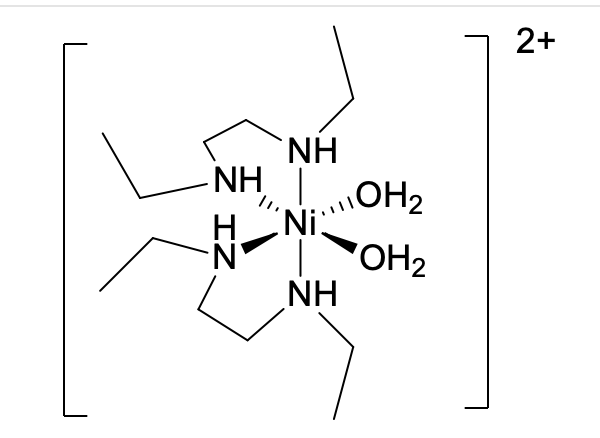
\includegraphics[width=0.4\linewidth]{foto/nieten2.png}
    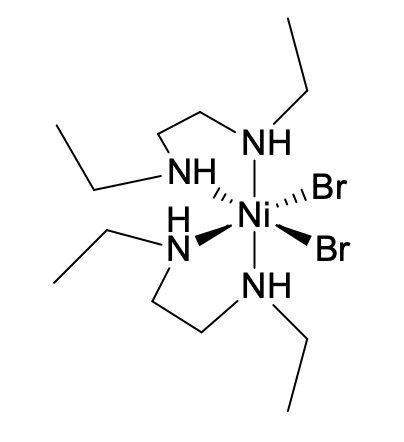
\includegraphics[width=0.265\linewidth]{foto/nietenbr2.png}
    \caption{A sinistra troviamo \ce{[Ni(Et2en)2(H2O)2]Br2 } mentre a destra \ce{[Ni(Et2en)2Br2]} }
    \label{fig:nieten}
\end{figure}



\subsubsection{Procedura sperimentale}

Abbiamo preparato una soluzione di bromuro di nichel sciogliendo $1.36 \mathrm{~g}$ di $\mathrm{NiBr}_2 \cdot 3 \mathrm{H}_2 \mathrm{O}$ in $30 \mathrm{~mL}$ di etanolo. Successivamente abbiamo aggiunto  $1.4 \mathrm{~mL}$ di $\mathrm{Et}_2 \mathrm{en}$\footnote{ Quantità corrispondente a 1.6 g prescritti nelle dispense}. Precipita un solido di colore verde acqua che dopo qualche ora dovrà essere filtrato su Buchner e lavato con etanolo. Lasciato seccare sul filtro sotto all'azione della pompa, lo si trasferisce in una provetta precedentemente pesata per poi essiccarlo sottovuoto. Dopo aver pesato la provetta contenente il sale ormai asciutto trasferisco, successivamente, metà del suo contenuto in un'altra provetta precedentemente pesata che colloco in stufa per disidratare il composto rimuovendo l'acqua dalla sfera di coordinazione interna. Infine, il giorno successivo si pesa la provetta e si calcola la perdita d'acqua.

\subsubsection{Commenti e osservazioni}
Una scarsa dimestichezza con le operazioni di filtrazione ci ha fatto terminare precocemente la filtrazione lasciando il solido sul filtro ancora bagnato\footnote{In parte è anche colpa della particelle del solido, che essendo molto piccole hanno trattenuto molta acqua e creato una pasta molto densa e corposa che ha rallentato l'essiccamento sul filtro}. Questo ha provocato la formazione di una pasta molto densa è appiccicosa che è rimasta su tutta l'attrezzatura riducendo la quantità di prodotto finale ottenuto.
Abbiamo notato un cambio colorazione successivo al trattamento del prodotto idrato in stufa. Una volta finito il processo di essiccamento si potevano distinguere le due porzioni; quella trattata e quella no.
\subsubsection{Calcoli e analisi dati}

Il numero di moli di \ce{NiBr2.3H2O} che occorrono sono
$$
n_{\mathrm{NiBr}_2}=\frac{1.36 \mathrm{~g}}{272.55 \mathrm{~g} / \mathrm{mol}}=4.990 \mathrm{~mmol}
$$
Sulle dispense erano riportata la massa da prelevare, avendo a disposizione una pipetta dobbiamo convertire il dato in un volume

\[ V = \frac{m}{\rho} = \frac{1.16\um{g}}{0.827 \um{g/mL}} = 1.4 \um{mL} \]


per \ce{Et2en} $\rho = 0.827 \um{g/mL}$
$$
n_{\mathrm{Et}_2 \mathrm{en}}=\frac{1.4 \mathrm{~mL} \cdot 0.827 \mathrm{~g} / \mathrm{mL}}{116.20 \mathrm{~g} / \mathrm{mol}}=9.96 \mathrm{~mmol}
$$
Poiché la stechiometria del prodotto è $1: 2$ si ricava che il reagente limitante è la N,N-dietiletilendiammina. 

Calcoliamo la resa 
\[ Y_\% = \frac{n_\text{pro}}{n_{\mathrm{NiBr}_2}}\cdot 100 \]

Le moli finali sono il rapporto massa della provettà piena di prodotto tolta la tara e la massa molare del prodotto.

\[ n_\text{pro} = \frac{m_{f} - m_{t}}{M_\text{pro}} 
 = \frac{ 17.1101\um{g} - 15.0134 \um{g}}{ 486.93 \um{g/mol}} =  \frac{2.097 \mathrm{~g}}{486.93 \mathrm{~g} / \mathrm{mol}}=4.306 \um{mmol}\]

\[ Y_\% = \frac{n_\text{pro}}{n_{\mathrm{NiCl}_2}}\cdot 100  = \frac{2 \cdot 4.306 \cdot 10^{-3} \mathrm{~mol}}{9.96 \cdot 10^{-3} \mathrm{~mol}} \cdot 100 =86.5 \%\]


Calcoliamo ora la perdita di peso della frazione lasciata in stufa. Abbiamo pesato $ 0.8751  \um{g} $ di composto e ci siamo segnati la tara   $ 20.7369\um{g}$. Dopo la disidratazione la massa della provetta era $ 21.6770 \um{g}$. La perdita netta di peso teorica è: 

\[ \Delta m =\frac{ 2\cdot M_{\ce{H2O}}}{M_{\text{pro}} } m_{\text{pesata}} \]

Vediamo che il $\Delta m$ sperimentale è 
\[ \Delta m = m_f -(m_{\text{tara}} +m_{\text{pro}}) = 21.6770 \um{g} - 20.7369 \um{g} - 0.8751   \um{g} = 0.065\um{g}\]
\subsection{Preparazione di {\ce{[Ni(NH3)6] }}}

\begin{figure}[ht!]
    \centering
    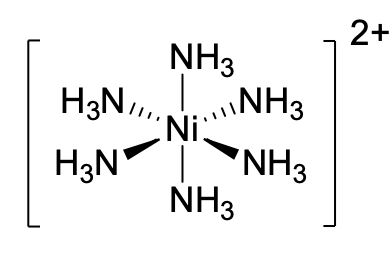
\includegraphics[width=0.3\linewidth]{foto/ninh3.png}
    \caption{Complesso \ce{[Ni(NH3)6] }}
    \label{fig:ninh3}
\end{figure}
\subsubsection{Procedura sperimentale}
Abbiamo preparato una soluzione di cloruro di nichel sciogliendo di $3.00$ g \ce{NiCl2} $\cdot$ 6\ce{H2O} 
in 5 mL di \ce{H2O} a caldo. Successivamente abbiamo aggiunto $5.8$ mL di \ce{NH4OH} concentrato. Si raffredda usando un bagno di ghiaccio si completa la precipitazione aggiungendo etanolo. Si filtra il precipitato su Buchner, si trasferisce in una provetta precedentemente pesata e si asciuga sotto vuoto. Si pesa il prodotto asciutto e si calcola la resa di reazione
\subsubsection{Commenti e osservazioni}
La reazione è avvenuta senza imprevisti. Dopo l'aggiunta dell'idrossido di ammonio si è subito notata la variazione di colore. Come si vede dai calcoli, si utilizza un largo eccesso di idrossido di ammonio in quanto la reazione di complessazione è un equilibrio, aggiungendo un reagente l'equilibro, verrà spostato verso la formazione dei prodotti. Il successivo raffreddamento e l'aggiunta di etanolo incentiveranno la formazione di prodotto e sarà rimosso dall'ambiente di reazione favorendo la complessazione. Il complesso è idrolabile se lasciato in acqua pura l'ammoniaca viene liberata e si riforma l'esaacquo-ione di partenza. Come per il complesso precedente abbiamo utilizzato il cloruro anidro quindi la massa effettiva di solido pesata era minore.




\subsubsection{Calcoli e analisi dei dati}
Come prima, il numero di moli di $\mathrm{NiCl}_2 \cdot 6 \mathrm{H}_2 \mathrm{O}$ che occorrono sono
$$
n_{\mathrm{NiCl}_2}=\frac{3.00 \mathrm{~g}}{237.70 \mathrm{~g} / \mathrm{mol}}=0.0126 \mathrm{~mol}
$$
che convertite in massa di \ce{NiCl2} anidro da pesare si trasformano in

\[  {m_{\ce{NiCl2}}} = n_{\mathrm{NiCl}_2} \cdot {M_{\ce{NiCl2}}} = 12.6 \text{mmol} \cdot 129.6  \ \text{g/mol} = 1.63 \text{g} \]

Calcoliamo le moli di ammoniaca aggiunte, sappiamo che una soluzione concentrata di idrossido di ammonio è circa $18$ M \cite{ammonia}, quindi in $5.8$ mL ci sono

\[ n_{\ce{NH3}} = C \cdot V = 18\um{mmol/mL} \cdot 5.8 \ \text{mL} = 104.4 \um{mmol} \]

Ora calcoliamo la resa sulle moli di nichel iniziali
\[ Y_\% = \frac{n_\text{pro}}{n_{\mathrm{NiCl}_2}}\cdot 100 \]

Le moli finali sono il rapporto massa della provettà piena di prodotto tolta la tara e la massa molare del prodotto.

\[ n_\text{pro} = \frac{m_{f} - m_{t}}{M_\text{pro}} 
 = \frac{17.7280 \um{g} - 15.1515\um{g} }{ 231.78 \um{g/mol}} = 0.01112 \um{mol}\]

\[ Y_\% = \frac{n_\text{pro}}{n_{\mathrm{NiCl}_2}}\cdot 100  = \frac{0.01112 \um{mol}}{0.0126 \um{mol}} \cdot 100 = 88.2\% \]
La resa concorda con quanto viene riportato in letteratura \cite{support}
\subsection{Caratterizzazione UV-VIS}
\subsubsection{Procedura sperimentale}
Si preparano 3 soluzioni circa 0.1 M dei tre sali portando a volume con acqua \ce{[Ni(en)3]Cl2.2H2O} e \ce{[Ni(Eten)2H2O]Br2}
mentre con \ce{NH4OH} 3 M \ce{[Ni(NH3)6]Cl2}\footnote{Come già detto \ce{[Ni(NH3)6]Cl2} si  idrolizza se sciolto in acqua.}
La polvere da pesare per ottenere una soluzione di quella concentrazione in un matraccio da 50 mL\footnote{Abbiamo fatto questa scelta di volume per non dover utilizzare troppo campione ma comunque mantenendo una quantità tale mantenere precisa la pesata. Per il \ce{[Ni(Eten)2H2O]Br2} abbiamo scelto un matraccio da 10 mL perché non avevamo abbastanza prodotto per fare l'analisi.}

\[ m_{\ce{[Ni(NH3)6]Cl2}} = C \cdot V_{\text{matraccio}} \cdot M_{\ce{[Ni(NH3)6]Cl2}}  = 0.1 \um{M} \cdot 50 \um{mL} \cdot 231.78 \um{g/mol} = 1.1589 \um{g} \]

\[ m_{\ce{[Ni(en)3]Cl2}} = C \cdot V_{\text{matraccio}} \cdot M_{\ce{[Ni(en)3]Cl2.2H2O}}  = 0.1 \um{M} \cdot 50 \um{mL} \cdot 345.92 \um{g/mol} = 1.7296 \um{g} \]

\[ m_{\ce{[Ni(Eten)2(H2O)2]Br2}} = C \cdot V_{\text{matraccio}} \cdot M_{\ce{[Ni(Eten)2(H2O)2]Br2}}  = 0.1 \um{M} \cdot 10 \um{mL} \cdot 486.93 \um{g/mol} = 0.4689\um{g} \]

In  \autoref{tab:pesate} sono presenti i valori pesati dei tre sali.
\subsubsection{Spettri}


\begin{figure}[ht!]
    \centering
    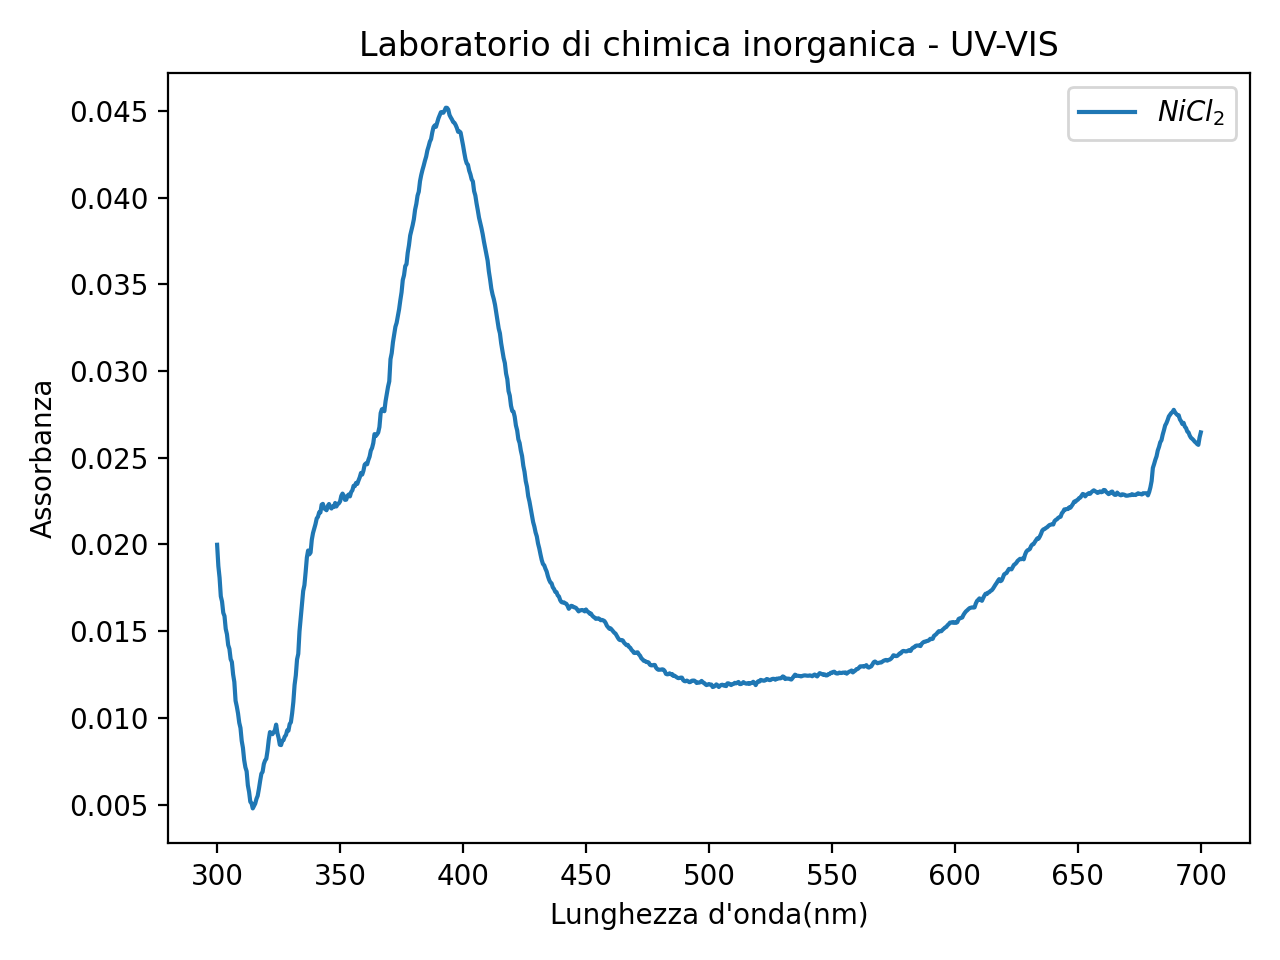
\includegraphics{Relazione/foto/nicl2uv.png}
    
    \caption{Spettro UV-VIS \ce{NiCl2} in acqua}
    \label{fig:nicl2uv}
\end{figure}

\begin{figure}[ht!]
    \centering
    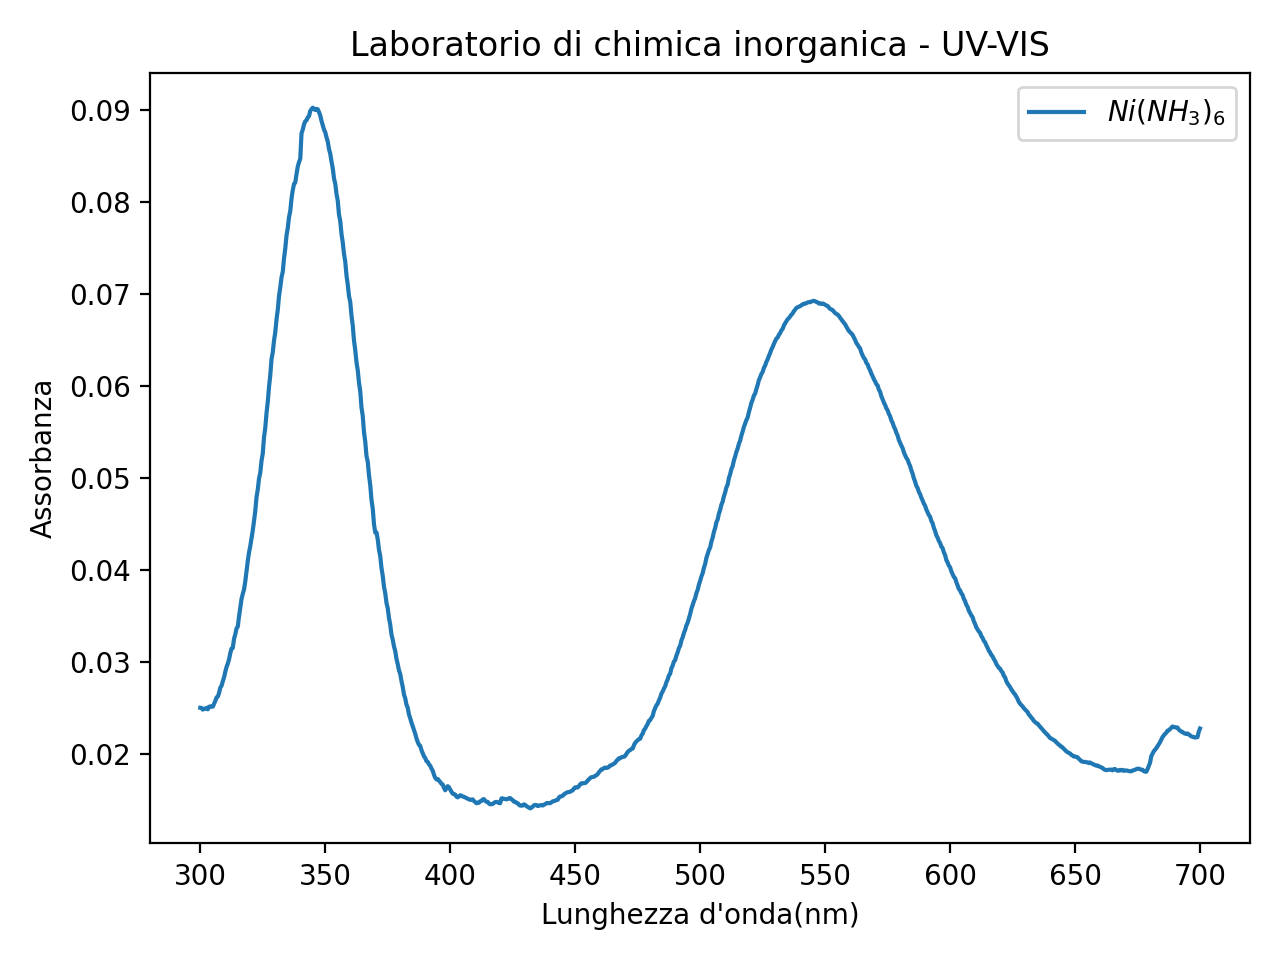
\includegraphics{Relazione/foto/ninh3uv.png}
    
    \caption{Spettro UV-VIS \ce{[Ni(NH3)6]Cl2} in acqua}
    \label{fig:ninh3uv}
\end{figure}
\begin{figure}[ht!]
    \centering
   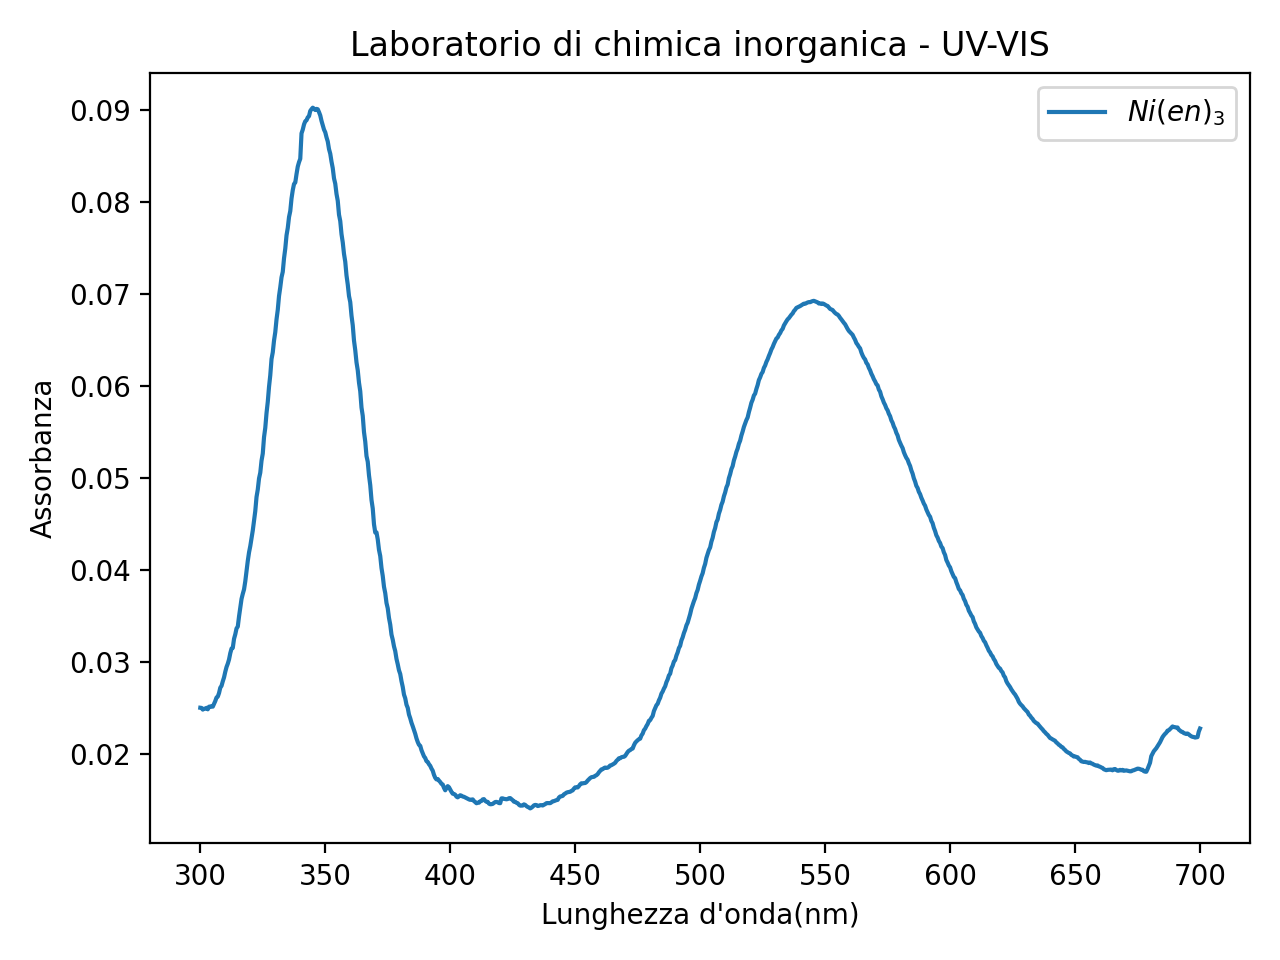
\includegraphics{Relazione/foto/Nienuv.png}
    \caption{Spettro UV-VIS \ce{[Ni(en)3]Cl2} in acqua}
    \label{fig:nienuv}
\end{figure}
I dati per lo spettro di \ce{[Ni(Eten)2(H2O)2]Br2} non sono stati persi, in \autoref{fig:NiEtenuv} è riportato lo spettro acquisito da un altro gruppo. Abbiamo, invece acquisito lo spettro del \ce{NiCl2} in acqua

\[ m_{\ce{NiCl2}} = C \cdot V_{\text{matraccio}} \cdot M_{\ce{NiCl2}}  = 0.1 \um{M} \cdot 50 \um{mL} \cdot 129.6 \um{g/mol} = 0.648 \um{g} \]
\begin{figure}[ht!]
    \centering
   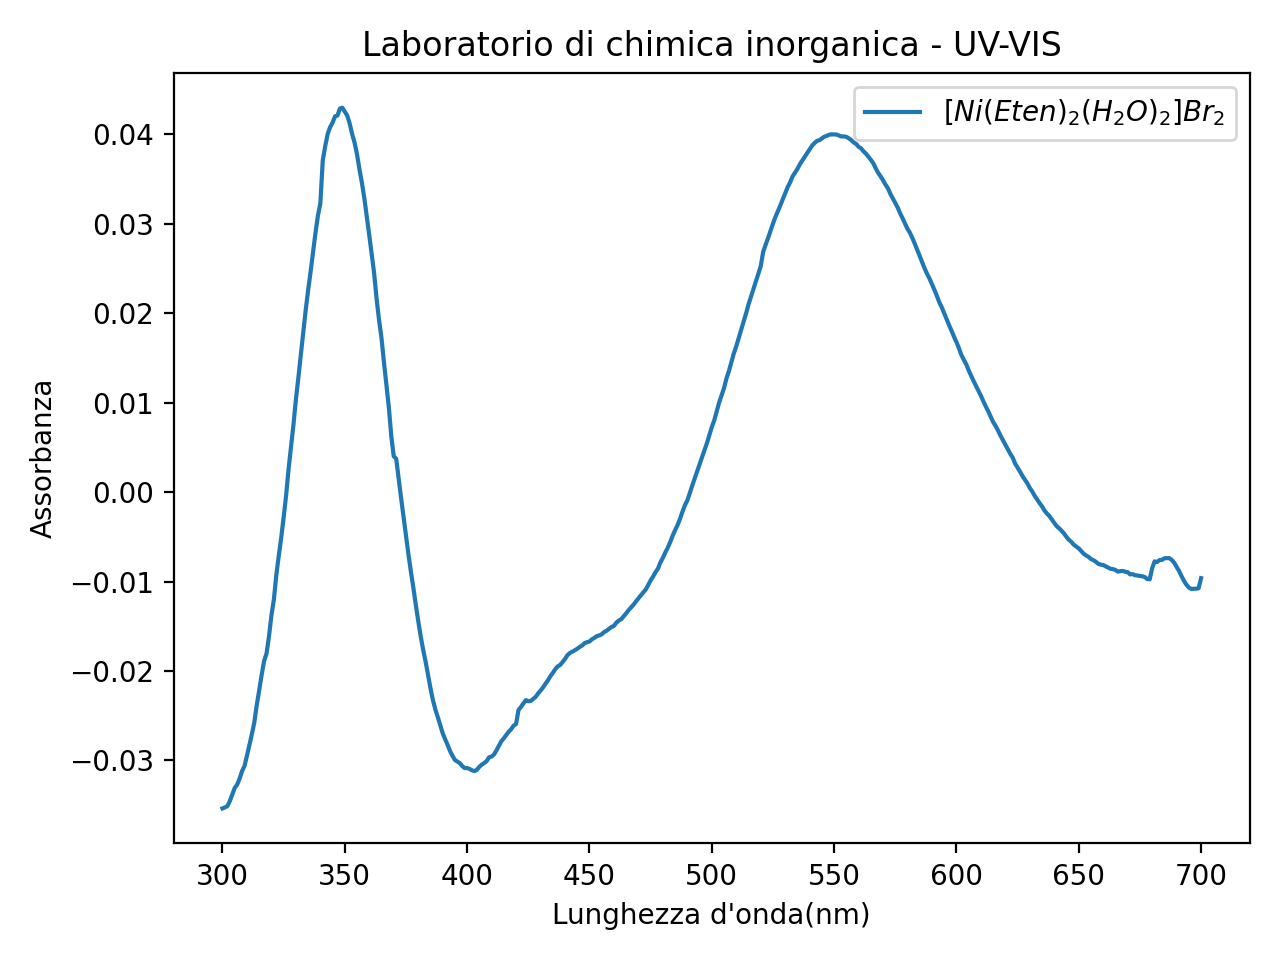
\includegraphics{Relazione/foto/Nibr2.png}
    \caption{Spettro UV-VIS \ce{[Ni(Eten)2(H2O)2]Br2} in acqua}
    \label{fig:NiEtenuv}
\end{figure}
\subsubsection{Commenti e osservazioni}
Confrontiamo gli spettri tenendo conto che il nichel(II) è un centro $d^8$. Pertanto, usando i diagrammi di Tanabe-Sugano, possiamo prevedere la presenza di tre bande di assorbimento relativamente  intense dovute alle tre transizioni spin-permesse dallo stato fondamentale ${ }^3 A_{2 g}$ verso agli stati eccitati ${ }^3 T_{2 g},{ }^3 T_{1 g}(F)$ e ${ }^3 T_{1 g}(P)$. Possiamo sfruttare proprio l'informazione spettroscopica per valutare quale sia lo splitting di campo cristallino indotto dalla presenza dei leganti. Se avessimo i massimi della banda a più bassa energia non ci sarebbe nessuna difficoltà in quanto l'energia corrisponderebbe proprio al $\Delta_o$. Purtroppo, non essendo visibile, dobbiamo arrangiarci con le altre due bande e con i diagrammi di Tanabe-Sugano. Ad esempio, per $\mathrm{Ni}\left(\mathrm{NH}_3\right)_6 \mathrm{Cl}_2$ possiamo calcolare il rapporto fra le energie delle due transizioni
$$
\frac{E_3 A_{2 g} \rightarrow{ }^3 T_{1 g}(P)}{E_3 A_{2 g} \rightarrow{ }^3 T_{1 g}(F)}=\frac{\lambda_F}{\lambda_P}=\frac{545 \mathrm{~nm}}{345 \mathrm{~nm}}=1.58
$$
Adesso, cercando sul diagramma di Tanabe-Sugano per un centro $d^8$ il valore di $\Delta_o / B$ per cui c'è questo stesso rapporto fra le ordinate degli stati coinvolti ricaviamo $\Delta_o / B=14.98$. Leggiamo inoltre dal grafico che la differenza in energia fra le due bande vale $13.40 \mathrm{E} / \mathrm{B}$. Ma poiché questa differenza di energia è nota dallo spettro, possiamo ricavare il valore dello splitting dovuto ai leganti come
$$
\Delta_o=\left[\frac{14.98}{13.40} \cdot\left(\frac{1}{345 \mathrm{~nm}}-\frac{1}{545 \mathrm{~nm}}\right)\right]^{-1}=841 \mathrm{~nm}
$$
Il risultato sembra ragionevole in quanto dalla porzione di banda che si vede nello spettro si può indovinare la presenza di un massimo proprio intorno a questa lunghezza d'onda. Ripetendo lo stesso procedimento per $\mathrm{Ni}\left(\mathrm{NH}_3\right)_6 \mathrm{Cl}_2$ si ottiene $\Delta_o=893 \mathrm{~nm}$ che corrisponde, come atteso, ad un'energia minore rispetto al caso precedente. Per \ce{[Ni(Eten)2(H2O)]Br2}  $\Delta_o = 857 $ nm. Il complesso di esaacquonichel è più complicato poiché presenta una banda sdoppiata dovuta, a quanto ho visto in letteratura, al fatto che i livelli ${ }^3 T_{1 g}(F)$ e ${ }^1 E_g$ siano quasi degeneri per il valore di splitting indotto dall'acqua e che quindi possano accoppiare fra loro. Non è quindi semplice decidere quale frequenza prendere, ma si possono ottenere valori di $\Delta_o$ compresi fra $800 \mathrm{~nm}$ e $1050 \mathrm{~nm}$\cite{nicheluv}.



\subsection{Caratterizzazione tramite misura magnetica}
Abbiamo eseguito 4 misure per ciascun composto alla bilancia Johnson Matthey. La costante della bilancia valeva $C = 1.087 \cdot 10^{-9}$ e la temperatura risultava di 24 °C.
I dati raccolti si possono trovare in \autoref{sec:dati} nella \autoref{tab:magnet}



\begin{table}[ht!]
\centering
\textbf{Risultati}

\begin{tabular}{lcc}
 \hline 
 Composto & $\chi (10^{-6})$[$\mathrm{cm^3/g}$]  & Incertezza    \\
\hline\hline 
 \multirow{4}{*}{$\left[\mathrm{Ni}\left(\mathrm{Et}_2 \mathrm{en}\right)_2\left(\mathrm{H}_2 \mathrm{O}\right)_2\right] \mathrm{Br}_2$} & 8.337 & .410 \\ 

& 8.191 & .355 \\
& 8.148 & .434 \\
&8.245& .403  \\
\hline
Media & 8.230 & \\
$\sigma$ & .057 & \\
\hline
 \multirow{4}{*}{ \ce{[Ni(en)3]Cl2}} & 9.625 & .513  \\ 
 & 9.675 & .454  \\
& 9.744 & .436  \\
& 9.624 & .514  \\ \hline
Media & 9.668 & \\
$\sigma$ & .056 & \\


 
\hline
\end{tabular}

\caption{Misure della suscettibilità magnetica con relativa incertezza. Deviazione standard e media delle misure}
\label{tab:magn}
\end{table}
Possiamo trovare i valori di suscettibilità dai valori misurati tramite la seguente formula:
\[\chi_s =\frac{L}{m}\left[C\left(R-R_0\right)\right]\]
Calcoliamo la suscettibilità magnetica molare tramite la seguente formula:

\[ \chi_m =  \chi_s M \]


\begin{table}[ht!]
\centering
\begin{tabular}{lcc}
 &\ce{[Ni(en)3]Cl2}    &  \ce{[Ni(Eten)2(H2O)2]Br2} \\ \hline
 [$\mathrm{cm^3/mol} \cdot $] $10^{-3}$ &  3.34  & 4.01\\
\end{tabular}
\end{table}
Si può assumere che la suscettibilità possa essere calcolata
\[ \chi'_m = \chi_m - \chi_{\ce{dia}}\]
in quanto il materiale è mesoscopicamente omogeneo. Inoltre, si può assumere in prima approssimazione che 
\[\chi_{\ce{dia}} = \sum_i \nu_i \chi_{\ce{dc}}\]
Con un po' di conti si può ricavare che\footnote{\url{https://github.com/mfiaschi5/labinorganica/blob/main/Magnetismo_nella_materia.pdf}}
\[ \frac{\mu}{\mu_B} = 2.828\sqrt{\chi'_m T}\]
Possiamo associare a questo il numero di elettroni spaiati al momento magnetico
\[ \frac{\mu}{\mu_B} = \sqrt{n(n+1)}\]

Dall'ultima equazione è quindi possibile ricavare il numero di elettroni spaiati del complesso $n$, che in particolare sarà espressa dalla seguente equazione:

\begin{equation}
   n = \frac{-1 + \sqrt{1+4(\frac{\mu}{\mu_b})^2}}{2} 
   \label{eq:n}
\end{equation}

ove la soluzione negativa è stata scartata in quanto priva di significato.

\begin{table}[ht!]
\centering
\begin{tabular}{l ccccc r}\hline
& \ce{en} & \ce{Cl} & \ce{H2O} & \ce{Eten} & \ce{Br} & Contributo totale \\
\hline\hline
Correzione diamagnetica($10^{-3})$ & 0.046 & -0.0234 & -0.013 & -0.073 & -0.0346 &  \\
$\nu_i$ \ce{[Ni(en)3]Cl2}  & 3 & 2 & 2 & 0 & 0&-0.2108 \\
 $\nu_i$ \ce{[Ni(Eten)2(H2O)2]Br2}& 0 & 0 & 2 & 2 & 2 & -0.2412\\\hline
\end{tabular}
\end{table}

\begin{table}[ht!]
\centering
\begin{tabular}{ccccc}
Composto& Temperatura[°C] & $\chi'_m(10^{-3})$ & $\mu$[$\mu_B$] & n \\
\hline
\ce{[Ni(en)3]Cl2} & 24 & 3.56 & 2.91 & 2.07 \\
\ce{[Ni(Eten)2(H2O)2]Br2} & 24 &  4.25& 3.17 & 2.33 \\
\end{tabular}
\end{table}


\section{Sintesi e caratterizzazione di \ce{Co(salen)}}
\subsection{Sintesi}
\subsubsection{Procedura sperimentale}
In un pallone da 250 mL, munito di tappo, di rubinetto a due vie e di agitatore magnetico, abbiamo introdotto 2.6 mL  di aldeide salicilica e 100 mL di alcool etilico 95\%, insieme a 0.82 mL  di etilendiammina. Abbiamo avuto pronta precipitazione della base di Schiff di colore giallo. Abbiamo preparato a parte una soluzione di 3.0 g  di \ce{Co(CH3COO)2. 4 H2O} in 30 mL di acqua deionizzata. Questa soluzione è stata posta in imbuto gocciolatore munito di tappo con rubinetto a due vie\footnote{Soluzione di colore rosso rubino}. Dopo quattro cicli di vuoto-azoto, abbiamo gocciolato lentamente (circa 30 minuti) la soluzione del sale di cobalto nel pallone contenente l'immina, mantenuto  sotto azoto a circa 60 °C. Abbiamo lasciato raffreddare a temperatura ambiente e abbiamo filtrato in atmosfera inerte con il filtro a colonna il precipitato , lavando con due porzioni da 20 mL  di acqua deionizzata disaereata ed con 20 mL con alcool etilico disaereato. Abbiamo seccato il solido sotto vuoto controllando dopo un giorno la stabilità del peso in un intervallo di circa un'ora. 
\subsubsection{Apparato sperimentale}
\label{sec:cosalenapp}
La richiesta di un'atmosfera controllata in cui far avvenire la reazione impone l'utilizzo di apparecchiature specifiche. In questo caso il montaggio e la preparazione dell'apparato sono di vitale importanza per la riuscita dell'esperimento. La prima operazione da compiere è quella di preparare il sistema presente sotto la cappa; per fare ciò dovremo compiere alcuni cicli vuoto azoto per essere sicuri che in tutta l'apparecchiatura non sia presente ossigeno. Successivamente si monta la vetreria e si procede a fare alcuni cicli vuoto-azoto anche su di essa. Le valvole e le giunzioni sono state fissate con elastici per garantire l'integrità della struttura. Tutto l'apparato è stato fissato con un morsetto all'intelaiatura metallica presente sotto cappa; per dare maggior supporto al sistema incastreremo sotto il pallone un mantello scaldante grazie all'aiuto di un elevatore.
\begin{figure}[h!]
    \centering
    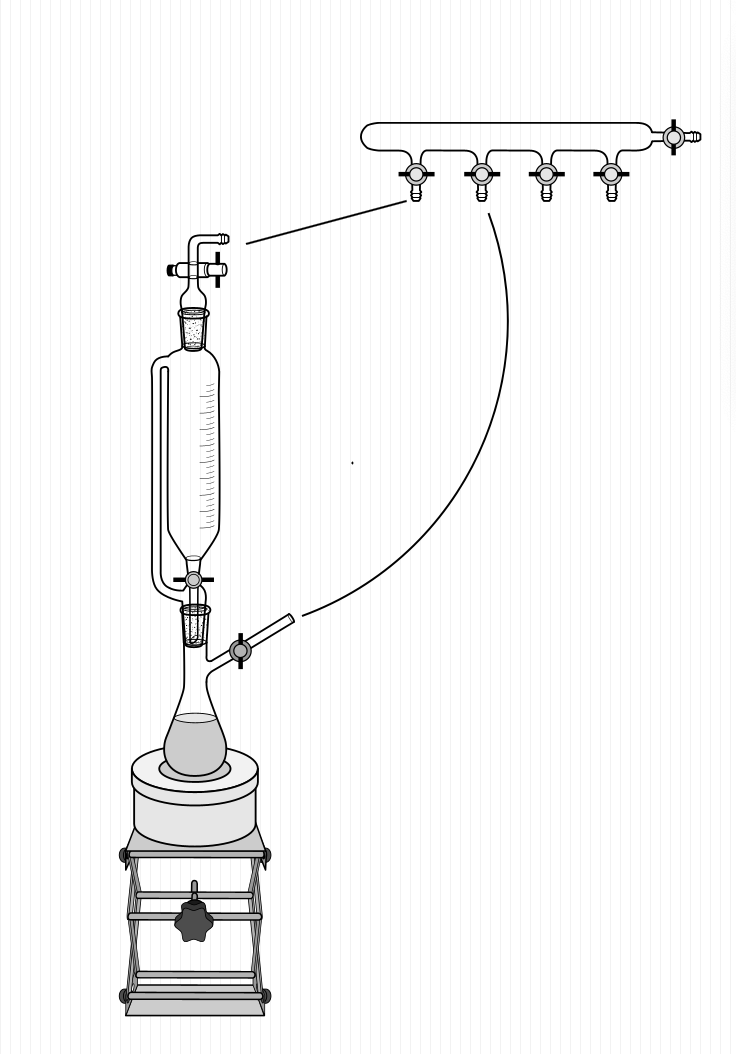
\includegraphics[width=0.4\linewidth]{foto/apparatosalen.png}
    \caption{Schema dell'apparato sperimentale usato per la sintesi. Nello schema mancano le valvole presenti sulle congiunzione tra i tubi e l'apparato. }
    \label{fig:my_label}
\end{figure}
Successivamente alla procedura di sintesi avviene la filtrazione che deve anch'essa essere svolta in atmosfera inerte. Questa fase è di fondamentale importanza per garantire una alta resa di reazione. Prepariamo un filtro a colonna e un adattatore maschio-maschio con coni smerigliati come mostrato in \autoref{fig:filtrosalen}. 
\begin{figure}[ht!]
    \centering
    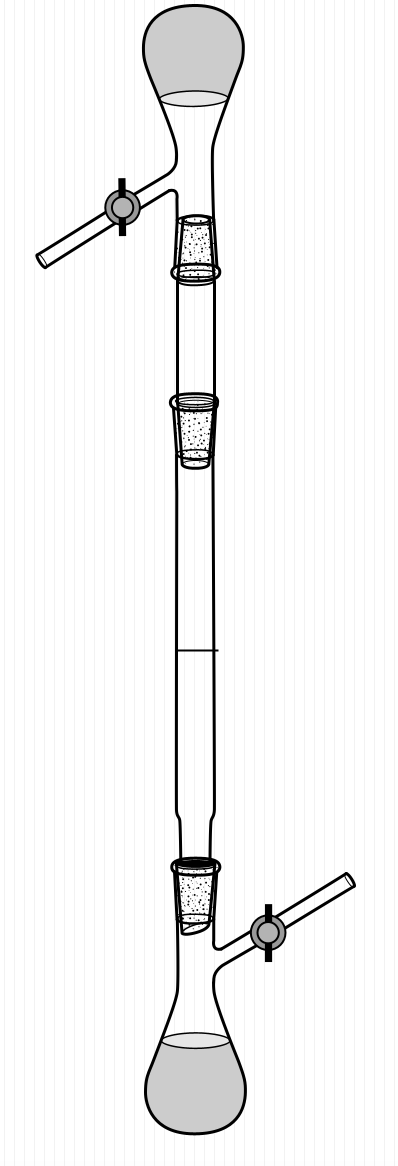
\includegraphics[width=0.15\linewidth]{foto/filtrazione.png}
    \caption{Schema dell'apparato di filtrazione. Di solido le valvole vanno tenute dalla stessa parte.}
    \label{fig:filtrosalen}
\end{figure}


Il pallone sotto va aggiunto successivamente e sarà quello contenente il prodotto da filtrare; prima dobbiamo tappare il sistema con una valvola e fare alcuni cicli di vuoto-azoto per bonificare l'apparato e sotto flusso di azoto collegare il sistema al pallone con il Co(salen)\footnote{Il pallone deve essere scollegato dall'imbuto gocciolatore e collegato al sistema sotto azoto }.


\subsubsection{Commenti e osservazioni}
Scaldare serve a sciogliere la base Schiff
DMSO passa la pelle e porta tutto dentro di te.

Pesata con provetta \cite{salenyield}


\subsubsection{Calcoli e analisi dei dati}

In partenza avevamo un numero di moli di reagenti pari a
\[ n_{\ce{Co(OAc)2}}=\frac{3 \mathrm{~g}}{345.58 \mathrm{~g} / \mathrm{mol}}= 12.0 \mathrm{~mmol} \]

\[ n_{\ce{AS}}=\frac{2.6 \mathrm{~mL} \cdot 1.146 \mathrm{~g} / \mathrm{mL} }{30.03 \mathrm{~g} / \mathrm{mol}}=24.6 \mathrm{~mmol} \]
\[ n_{en}=\frac{0.84 \mathrm{~mL} \cdot 0.899 \mathrm{~g} / \mathrm{mL}}{60.10 \mathrm{~g} / \mathrm{mol}}=12.6 \mathrm{~mmol} \]

Considerando quindi la stechiometria $1: 2: 1$ notiamo che il sale è il reagente limitante. 



Calcoliamo la resa 
\[ Y_\% = \frac{n_\text{pro}}{n_{\ce{[Co(en)3]Cl3}}}\cdot 100 \]

Le moli finali sono il rapporto massa della provettà piena di prodotto tolta la tara e la massa molare del prodotto.

\[ n_\text{pro} = \frac{(m_{f} - m_{t})}{M_\text{pro}} 
 = \frac{ 18.8692 \um{g} - 15.1226 \um{g} }{ 325.23 \um{g/mol}} =  \frac{3.7466 \mathrm{~g}}{325.23 \mathrm{~g} / \mathrm{mol}}=11.5 \um{mmol}\]

\[ Y_\% = \frac{n_\text{pro}}{n_{\ce{Co(salen)}}}\cdot 100  = \frac{  11.5 \cdot 10^{-3} \mathrm{~mol}}{12.0 \cdot 10^{-3} \mathrm{~mol}} \cdot 100 =96.0\%\]


\subsection{Spettro IR}


\subsubsection{Preparazione del campione}
Una punta di spatola di campione è stata messa in un mortaio con circa 2 goccie nujol e pestellata fino a completa omogenizzazione.  Su una finestra di cloruro di sodio viene messa una piccola porzione di miscela, con un'altra finestra si distribuisce e si copre in modo tale da poter essere inserita nell'apposito stand. Si inserisce il tutto nello strumento e si legge lo spettro. Infine, l'apparecchiatura viene smontata, le finestre vengono pulite con iso-propanolo  e lucidate su un panno usando come abrasivo dell'allumina.
\subsubsection{Interpretazione dello spettro}

NaCl assorbe sotto i 1200 cm
\begin{figure}[ht!]
    \centering
    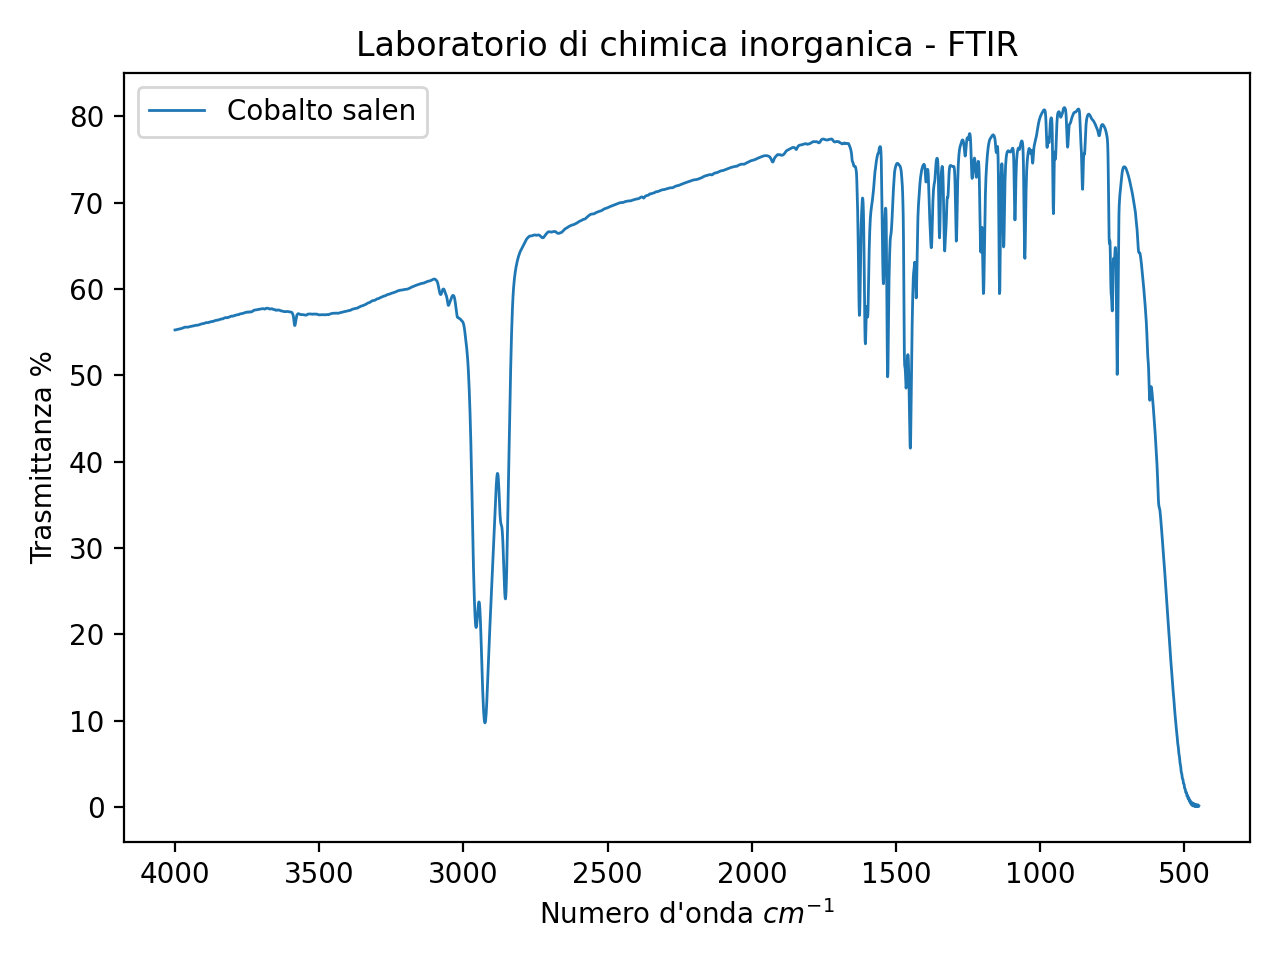
\includegraphics{Relazione/foto/FTIRsalen.png}
    \caption{Spettro FTIR del cobalto salen disperso nel jugol}
    \label{fig:FTIRsalen}
\end{figure}
\subsection{Assorbimento del diossigeno}
Abbiamo infine introdotto una piccola quantità di \ce{Co(salen)} finemente polverizzato in un becher e in cui abbiamo anche aggiunto circa 15 mL di DMSO. Abbiamo lasciato sotto agitazione per una notte. Abbiamo notato una variazione di colore della soluzione, la miscela ha perso l'iniziale sfumatura rossiccia diventando di color nero antracite. Abbiamo filtrato sottovuoto la soluzione. Abbiamo aggiunto parte del precipitato presente sul filtro in 10 mL di cloroformio. Abbiamo notato il ritorno del colore rosso segno della deossigenazione del complesso.


\section{Sintesi e caratterizzazione con 1H NMR di \ce{[Co(dinosar)]Cl3}}
\subsection{Sintesi \ce{[Co(en)3]Cl3}}
\subsubsection{Procedura sperimentale}
Abbiamo preparato una prima soluzione disciogliendo 6.02 g di \ce{CoCl2.6 H2O} in 17.5 mL circa d’acqua prelevata con un cilindro graduato. In contemporaneamente, abbiamo sciolto in un altro becher 5 mL (4.5 g) di etilendiammina in 12.5 mL di acqua. Quindi abbiamo acidificato la soluzione di etildiammina con 4.5 mL di acido cloridrico 6 M in un bagno di ghiaccio. Abbiamo unito le due soluzioni e abbiamo aspettato mezz’ora che avvenisse la complessazione. In seguito abbiamo aggiunto goccia a goccia 5.0 mL di acqua ossigenata al 30\% per ossidare il centro metallico. Al termine dell’effervescenza abbiamo svaporato a 30 mL e aggiunto lentamente 30 mL di HCl 12 M e 60 mL di etanolo. È precipitato un sale giallo ocra che abbiamo filtrato su Buchner, lavato con etanolo (3 × 10 mL). Abbiamo raccolto il prodotto in una provetta precedentemente pesata e l'abbiamo seccato sottovuoto.

\subsubsection{Commenti e osservazioni}
Durante l'acidificazione dell'etildiammina con HCl abbiamo notato la formazione di fumi bianchi. Questi si presume dovuti all'etildiammonio cloruro prodotto dalla reazione dell'acido cloridrico gassoso con etildiammina passata in fase gas per il riscaldamento della soluzione dovuto all'esotermicità della reazione di acidificazione. L'acqua ossigenata utilizzata era stata tenuta in frigo, i perossidi sono sostanze sensibili e tendono a decomporsi.


\subsubsection{Calcoli e analisi dei dati}
In partenza avevamo un numero di moli di reagenti pari a
$$
\begin{gathered}
n_{\mathrm{CoCl}_2}=\frac{6.00 \mathrm{~g}}{237.93 \mathrm{~g} / \mathrm{mol}}=0.0253 \mathrm{~mol} \\
n_{\mathrm{en}}=\frac{5 \mathrm{~mL} \cdot 0.899 \mathrm{~g} / \mathrm{mL}}{60.10 \mathrm{~g} / \mathrm{mol}}=0.07479 \mathrm{~mol}
\end{gathered}
$$
La stechiometria della reazione è 1 : 3 notiamo che il reagente limitante è l'etilendiammina\footnote{E' il reagente limitante per poco. }.
Calcoliamo la resa 
\[ Y_\% = \frac{n_\text{pro}}{n_{\mathrm{CoCl}_2}}\cdot 100 \]

Le moli finali sono il rapporto massa della provettà piena di prodotto tolta la tara e la massa molare del prodotto.

\[ n_\text{pro} = \frac{(m_{f\#1} - m_{t\#1})+(m_{f\#2} - m_{t\#2})}{M_\text{pro}} 
 = \frac{ 3.7564 \um{g} + 4.1124 \um{g} }{ 345.58 \um{g/mol}} =  \frac{7.8688 \mathrm{~g}}{345.58 \mathrm{~g} / \mathrm{mol}}=22.77 \um{mmol}\]

\[ Y_\% = \frac{n_\text{pro}}{n_{en}}\cdot 100  = \frac{3 \cdot 22.77 \cdot 10^{-3} \mathrm{~mol}}{74.79 \cdot 10^{-3} \mathrm{~mol}} \cdot 100 =91.3\%\]


\subsection{Sintesi \ce{[Co(dinosar)]Cl3}}
\subsubsection{Procedura sperimentale}
Abbiamo sciolto $2.45 \mathrm{~g}$ esatti del prodotto del passaggio precedente in $25 \mathrm{~mL}$ di acqua con $1.20 \mathrm{~g}$ di carbonato di sodio. Abbiamo quindi aggiunto $18 \mathrm{~mL}$ di formaldeide al $40 \%$ prelevata con un cilindro e $2.5 \mathrm{~mL}$ (circa $2.8 \mathrm{~g}$) di nitrometano. Dopo aver lasciato la soluzione a temperatura ambiente per qualche ora l'abbiamo riscaldata per un'altra ora al minimo della piastra elettrica. Abbiamo quindi filtrato su Buchner e recuperato il precipitato arancione che abbiamo ricristallizzato da una soluzione in $\mathrm{HCl} $ 3M. Infine, dopo aver aggiunto etanolo come non solvente abbiamo filtrato su Buchner, seccato all'aria, trasferito in una provetta di massa nota e seccato sottovuoto.
\subsubsection{Commenti e osservazioni}



\subsubsection{Calcoli e analisi dei dati}
In partenza avevamo un numero di moli di reagenti pari a
\[ n_{\ce{[Co(en)3]Cl3}}=\frac{2.45 \mathrm{~g}}{345.58 \mathrm{~g} / \mathrm{mol}}= 7.090 \mathrm{~mmol} \]

\[ n_{\mathrm{HCOH}}=\frac{18 \mathrm{~mL} \cdot 1.09 \mathrm{~g} / \mathrm{mL} \cdot 40 \%}{30.03 \mathrm{~g} / \mathrm{mol}}=0.26 \mathrm{~mol} \]
\[ n_{\mathrm{CH}_3 \mathrm{NO}_2}=\frac{2.5 \mathrm{~mL} \cdot 1.127 \mathrm{~g} / \mathrm{mL}}{61.04 \mathrm{~g} / \mathrm{mol}}=0.0462 \mathrm{~mol} \]

Considerando quindi la stechiometria $1: 6: 2$ notiamo che il complesso il reagente limitante. Abbiamo ottenuto $ 2.675 \mathrm{~g}$ di prodotto



Calcoliamo la resa 
\[ Y_\% = \frac{n_\text{pro}}{n_{\ce{[Co(en)3]Cl3}}}\cdot 100 \]

Le moli finali sono il rapporto massa della provettà piena di prodotto tolta la tara e la massa molare del prodotto.

\[ n_\text{pro} = \frac{(m_{f} - m_{t})}{M_\text{pro}} 
 = \frac{ 17.7611 \um{g} - 15.0861 \um{g} }{ 539.73 \um{g/mol}} =  \frac{2.675 \mathrm{~g}}{539.73 \mathrm{~g} / \mathrm{mol}}=4.96 \um{mmol}\]

\[ Y_\% = \frac{n_\text{pro}}{n_{\ce{[Co(en)3]Cl3}}}\cdot 100  = \frac{ \cdot 4.96 \cdot 10^{-3} \mathrm{~mol}}{7.09 \cdot 10^{-3} \mathrm{~mol}} \cdot 100 =70.0\%\]

\subsection{Spettro NMR}



\begin{figure}
    \centering
    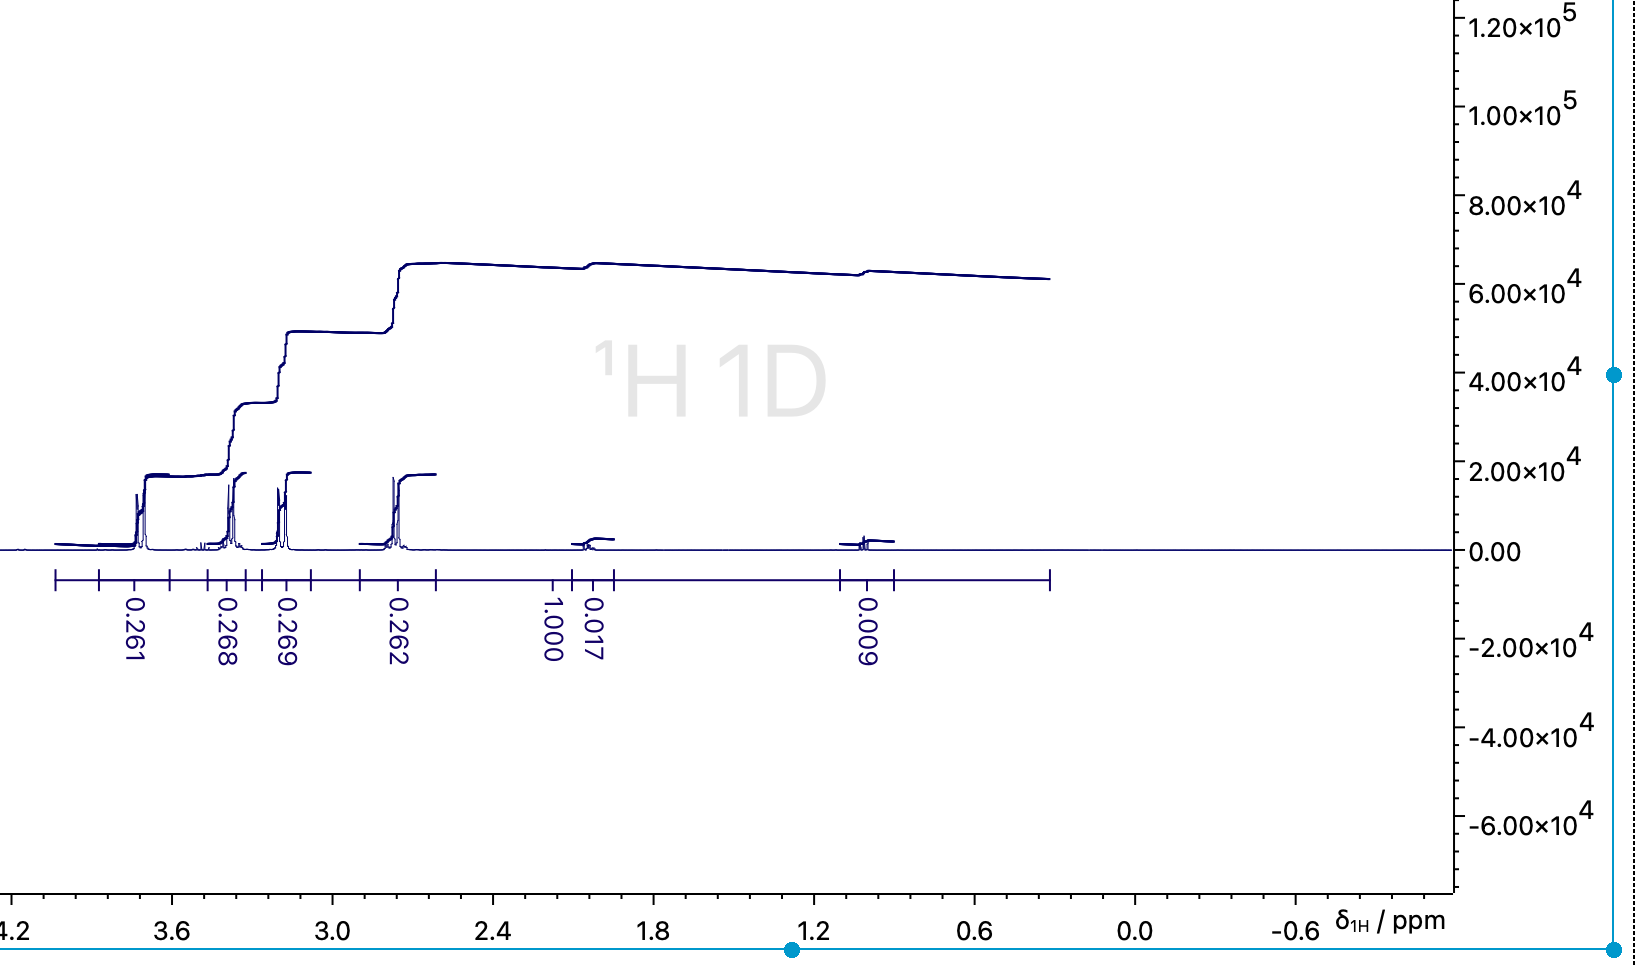
\includegraphics[width=0.8\linewidth]{Relazione/foto/Dinosar_integration_zoom.png}
    \caption{Caption}
    \label{fig:dinosarint}
\end{figure}



\begin{figure}
    \centering
    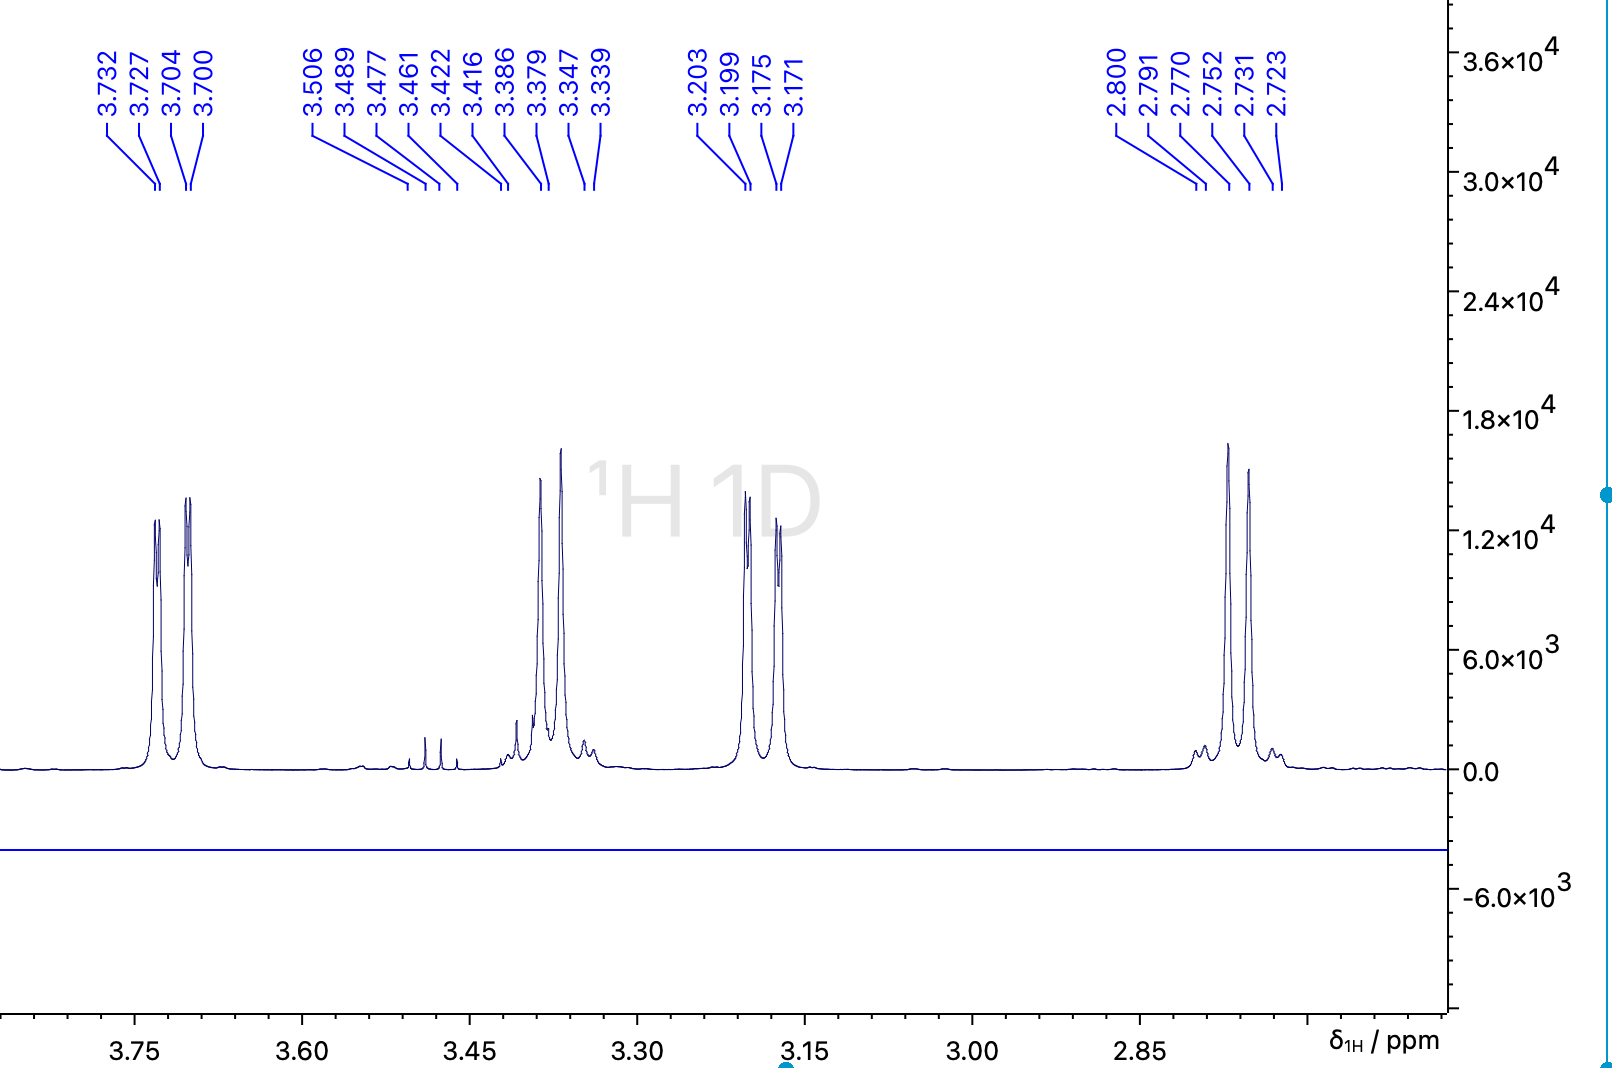
\includegraphics[width=0.8\linewidth]{Relazione/foto/Dinosar_peak_calc.png}
    \caption{Caption}
    \label{fig:dinosarpeakcalc}
\end{figure}

nmr i piccoli picchi posso essere dovuti all'etanolo di lavaggio


\section{Sintesi di \ce{[Cr2(OAc)4].2H2O}}
\subsection{Sintesi}
\subsubsection{Procedura sperimentale}

Iniziamo pesando 1.0 g di  bicromato di potassio. Successivamente, pesiamo 5.0 g di zinco polvere e trasferiamo sia il bicromato che lo zinco in un Schlenk precedentemente posto in atmosfera di azoto. In un altro Schlenk, anch'esso in atmosfera di azoto, sciogliamo 4,5 g di \ce{Na(OAc).3H2O} in 4 mL di acqua disareata, scaldando leggermente per ottenere completa dissoluzione. Sotto flusso di azoto abbiamo aggiunto 10 mL di HCl concentrato (12 M) goccia a goccia  nello Schlenk contenente il bicromato e lo zinco.
Lo zinco è cominciato a reagire immediatamente con l’acido liberando idrogeno. Abbiamo continuato l’aggiunta dell’acido, accertandoci di non produrre troppa effervescenza. Abbiamo aspettato per circa 15 minuti finché la soluzione ha smesso di produrre gas e non è diventata di colore blu zaffiro. Giunti a questo punto abbiamo connesso i due contenitori tramite un filtro ad Oliva, accertandosi che in entrambi fosse aperto l'azoto, aiutandosi con un sostengo abbiamo travasato la soluzione di \ce{Cr^{2+}} in quella di acetato. Alla formazione di un solido rosso abbiamo aspettato alcuni minuti per poi immergere il contenitore in un bagno di ghiaccio per una dozzina di minuti.
Infine, abbiamo filtrato il solido su un filtro a colonna in atmosfera di azoto
e l'abbiamo lasciato seccare sotto vuoto per una notte.






\subsubsection{Apparato sperimentale}
L'apparato di sintesi è composto da due tubi Schlenk, un filtro a oliva e un adattatore maschio-maschio\footnote{Quest'ultimo non è presente in figura ma nell'apparato originale era presente.}

Prima si monta un tubo Schlenk vi si pongono le polveri e si fanno un po' di cicli vuoto-azoto. Si bonifica dall'aria anche la sezione che comporrà la parte inferiore dell'apparato tappando l'estremità libera con una valvola analogamente a come fatto con il filtro nella \autoref{sec:cosalenapp}. Successivamente prepariamo la soluzione mantenendo tutto sotto flusso di azoto. Aiutandosi con un sostegno incliniamo entrambi i pezzi fino a raggiungere un posizione quasi orizzontale, sigilliamo e trasferiamo il contenuto del tubo contenente il cromo nella soluzione di acetato. Sotto azoto togliamo il filtro e l'altro tubo e sostituiamo con un tappo. 

Per le operazioni di filtraggio invece procederemo come già visto in \autoref{sec:cosalenapp}.



\begin{figure}[ht!]
    \centering
    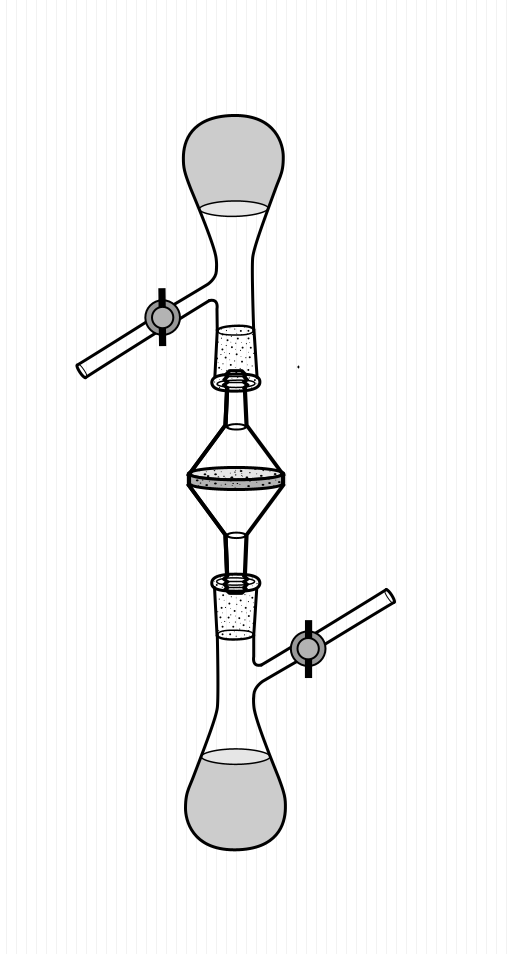
\includegraphics[width=0.3\linewidth]{foto/apparatooliva.png}
    \caption{Schema apparato di sintesi. Anche in questo caso le valvole vanno tenute preferibilmente dalla stessa parte}
    \label{fig:cracetao}
\end{figure}


\subsubsection{Commenti e osservazioni}

Bisogna fare particolare attenzione quando si maneggiano i bicromati in quanto sono molto tossici\footnote{Domanda forse ingenua: perché non abbiamo direttamente usato un sale di cromo(III) che è meno tossico e cancerogeno? In teoria avremo consumato anche meno zinco  \cite{cancer}.}. 
Formazione di un solido rosso dopo l'aggiunta della soluzione di cromo(II) a quella di acetato. 
Il solido asciutto e relativamente stabile all'aria ma comunque si degrada con il tempo. A differenza del cobalto salen in questo caso abbiamo adottato dei tubi Schlenk. Questa è una precauzione necessaria per salvaguardare le linee Schlenk in quanto, durante la reazione avviene la produzione di \ce{H2} che potrebbe creare schiume che sviluppandosi in altezza potrebbero arrivare alle linee dei gas entrando nei tubi e trasportandovi l'acido. Usando i tubi al posto dei palloni e aggiungendo cautamente l'acido questa problematica viene risolta.


\subsubsection{Calcoli e analisi dei dati}
In partenza avevamo un numero di moli pari a


\[   n_{\ce{K2Cr2O7}} = \frac{m_{\ce{K2Cr2O7}}}{M_{\ce{K2Cr2O7}}} = \frac{1 \um{g}}{294.19 \um{g/mol}} = 3.40 \um{mmol}\]

\[   n_{\ce{Zn}} = \frac{m_{\ce{Zn}}}{M_{\ce{Zn}}} = \frac{5 \um{g}}{65.41 \um{g/mol}} = 76.4 \um{mmol}\]


Il rapporto stechiometrico 1:2  quindi il notiamo che lo zinco è nettamente in eccesso. La resa verrà calcolata sulle moli di cromato.


Calcoliamo la resa 
\[ Y_\% = \frac{n_\text{pro}}{n_{\ce{Cr2(OAc)4.3H2O}}}\cdot 100 \]

Le moli finali sono il rapporto massa della provettà piena di prodotto tolta la tara e la massa molare del prodotto.

\[ n_\text{pro} = \frac{(m_{f} - m_{t})}{M_\text{pro}} 
 = \frac{ 17.6259 \um{g} - 15.0654 \um{g} }{ 588.40 \um{g/mol}} =  \frac{2.560 \mathrm{~g}}{588.40 \mathrm{~g} / \mathrm{mol}}=3.247 \um{mmol}\]

\[ Y_\% = \frac{n_\text{pro}}{n_{\ce{[Co(en)3]Cl3}}}\cdot 100  = \frac{ \cdot 3.247 \cdot 10^{-3} \mathrm{~mol}}{3.40 \cdot 10^{-3} \mathrm{~mol}} \cdot 100 =95.5\%\]


\section{Sintesi e caratterizzazione con 1H NMR di \ce{HCo[P(OPh)3]4}}
\subsection{Sintesi}
\subsubsection{Procedura sperimentale}
Abbiamo sciolto $0.5 \mathrm{~g}$ di nitrato di cobalto (II) esaidrato in $10 \mathrm{~mL}$ di etanolo e abbiamo aggiunto tramite pipetta graduata $2.5 \mathrm{~g}$ (circa $2.1 \mathrm{~mL}$) di trifenilfosfito. Abbiamo preparato a parte una soluzione di $0.20 \mathrm{~g}$ di sodio boroidruro in $5.0 \mathrm{~mL}$ di etanolo e quindi aggiunto goccia a goccia quest'ultima soluzione alla precedente su un intervallo di oltre mezz'ora. Il colore della soluzione vira dal rosso al giallo. Quindi filtriamo su Buchner e laviamo con etanolo, acqua e metanolo. Ridissolviamo il precipitato in $15 \mathrm{~mL}$ di diclorometano e poi con difficoltà filtriamo su Buchner per eliminare le impurità indissolte. Infine, riprecipitiamo con etanolo e raccolgliamo il complesso idrurico filtrando su Buchner.
\subsubsection{Commenti e osservazioni}

Durante l'aggiunta potevamo notare che nell'intorno del punto di contatto tra la goccia di sodioboroidruro e la soluzione si formava una zona bruna. Questo può essere causato dalla formazione di particelle di cobalto\cite{cored}.
Le dimensioni delle particelle di cobalto prodotte dipendono sensibilmente da una molteplicità di fattori diversi, questo spiega anche il fatto che per ogni gruppo le miscele avevano colori variabili. Nella zona dove avveniva l'immissione della soluzione 
 la concentrazione di \ce{NaBH4} era elevata e le particelle prodotte avevano dimensioni mesoscopiche dando alla soluzione un colore bruno. Nelle zone dove il sodioboroidruro era presente in minor quantità la dimensione delle particelle era minore, questo poteva produrre effetti di cambio di colore. Infatti, il colore di una sospensione di nanoparticelle di un metallo dipende dalle dimensioni di quest'ultime. 
La soluzione di etanolo dopo la notte aveva preso una colorazione sul verde acqua. Probabilmente questo è dovuto al fatto che il filtro non era stato lavato correttamente e parte dell'acido cloridrico usato dal gruppo precedente per la pulizia era rimasto nei pori e aveva trasformato parte dell'idruro in cloruro.
\subsubsection{Calcoli e analisi dei dati}



In partenza avevamo un numero di moli di reagenti pari a
\[ n_{\ce{Co(NO3)2.6H2O}}=\frac{0.5 \mathrm{~g}}{291.03 \mathrm{~g} / \mathrm{mol}}= 1.72 \mathrm{~mmol} \]

\[ n_{\ce{P(OPh)3}}=\frac{2.1 \mathrm{~mL} \cdot 1.184 \mathrm{~g} / \mathrm{mL} }{310.28 \mathrm{~g} / \mathrm{mol}}= 8.057 \mathrm{~mmol} \]

\[ n_{\ce{NaBH4}}=\frac{0.2 \mathrm{~g}  }{37.83 \mathrm{~g} / \mathrm{mol}}= 5.287 \mathrm{~mmol} \]

Considerando quindi la stechiometria $1: 3: 1$ notiamo che il sale di cobalto è il reagente limitante. 



Calcoliamo la resa 
\[ Y_\% = \frac{n_\text{pro}}{n_{\ce{Co(NO3)2.6H2O}}}\cdot 100 \]

Le moli finali sono il rapporto massa della provettà piena di prodotto tolta la tara e la massa molare del prodotto.

\[ n_\text{pro} = \frac{(m_{f} - m_{t})}{M_\text{pro}} 
 = \frac{ 15.6794 \um{g} - 15.0190 \um{g} }{ 1301.02 \um{g/mol}} =  \frac{0.6604 \mathrm{~g}}{1301.02 \mathrm{~g} / \mathrm{mol}}=0.508 \um{mmol}\]

\[ Y_\% = \frac{n_\text{pro}}{n_{\ce{HCo(OPh)3}}}\cdot 100  = \frac{  0.508 \cdot 10^{-3} \mathrm{~mol}}{1.72 \cdot 10^{-3} \mathrm{~mol}} \cdot 100 =29.5\%\]

\subsection{Spettro NMR}


\begin{figure}
    \centering
    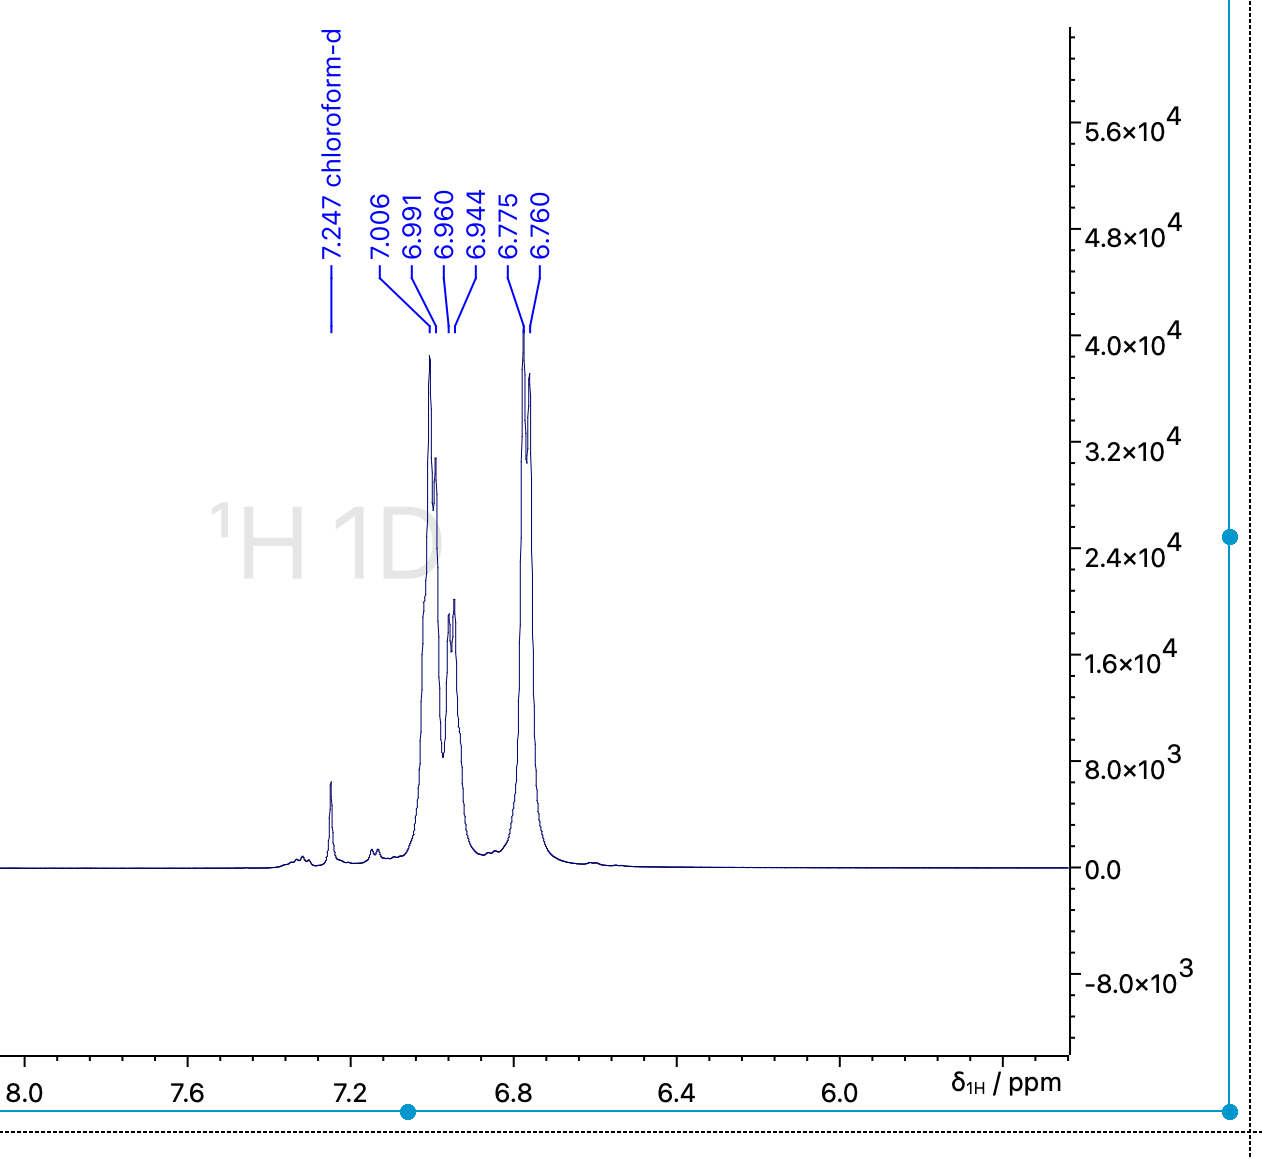
\includegraphics[width=0.8\linewidth]{Relazione/foto/CoH_aromaticpeak_calc_zoom.png}
    \caption{Caption}
    \label{fig:coharomaticzoom}
\end{figure}

\begin{figure}
    \centering
    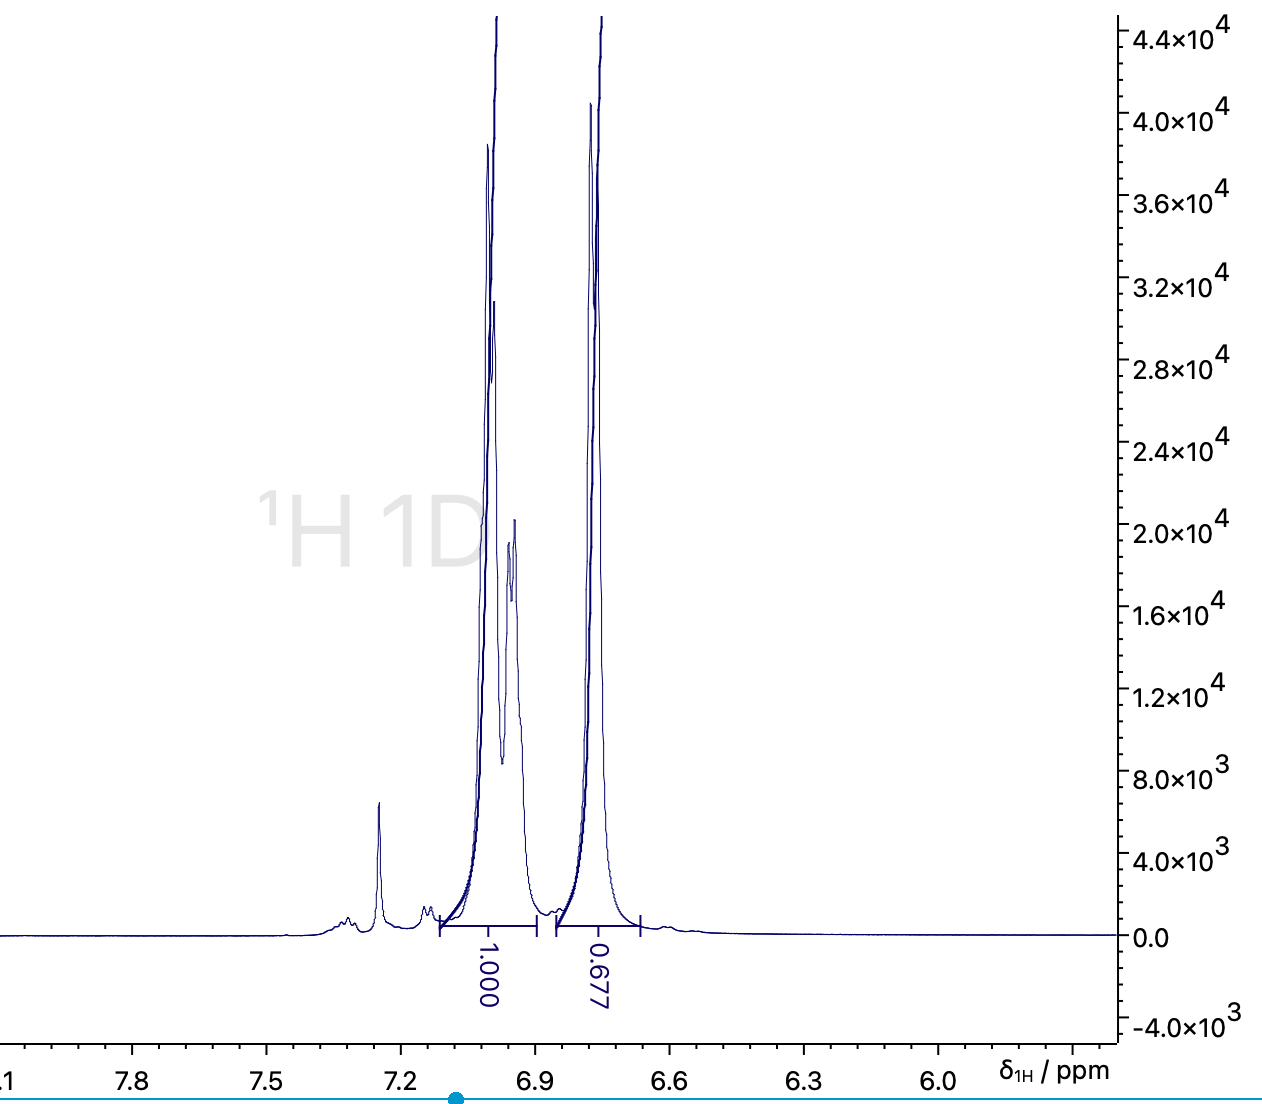
\includegraphics[width=0.8\linewidth]{Relazione/foto/CoH_aromaticpeak_right.png}
    \caption{Caption}
    \label{fig:my_label}
\end{figure}


\begin{figure}
    \centering
    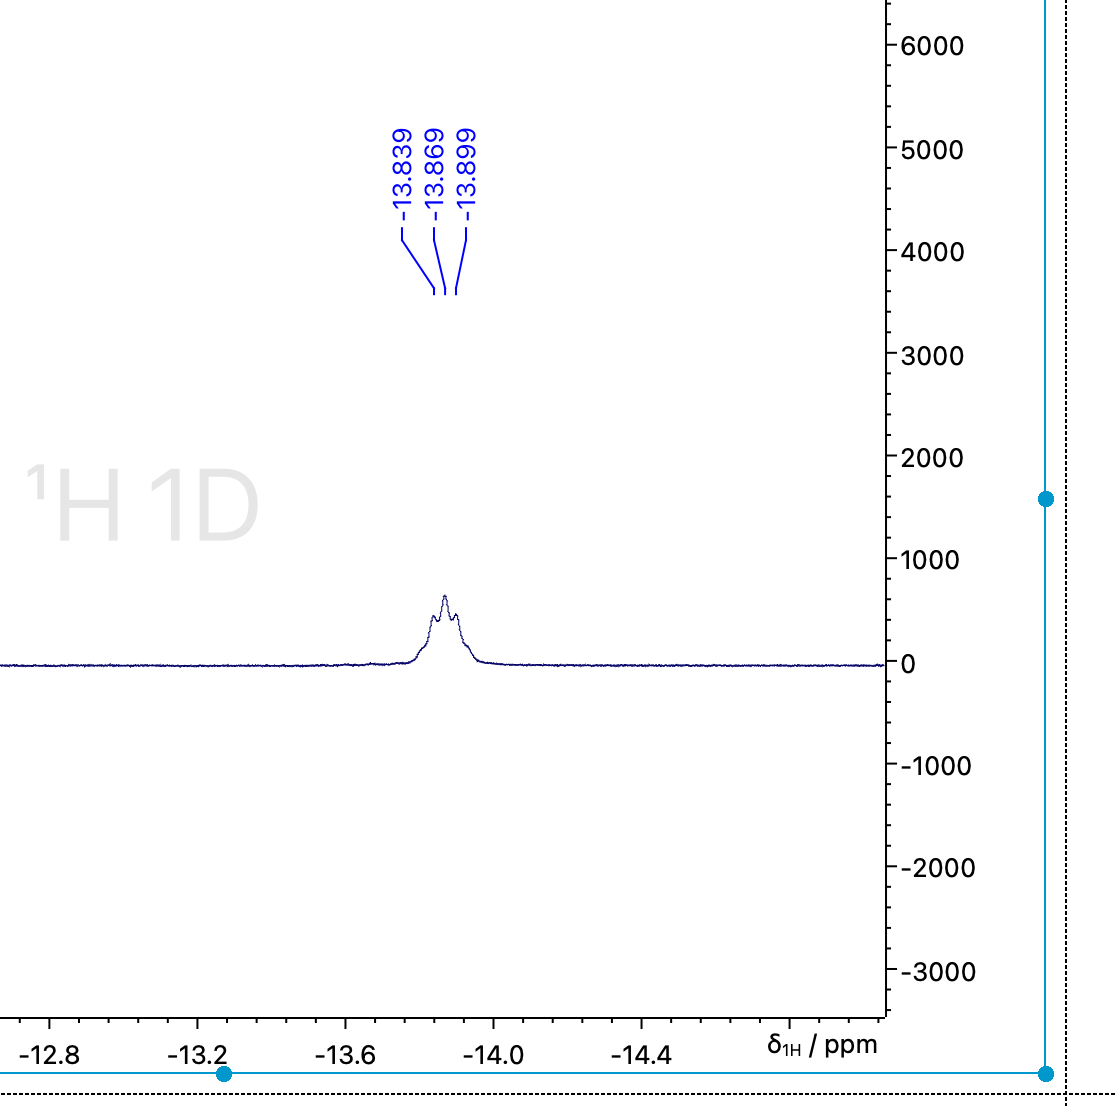
\includegraphics[width=0.8\linewidth]{Relazione/foto/CoH_hydridepeak_calc.png}
    \caption{Caption}
    \label{fig:my_label}
\end{figure}
\begin{figure}
    \centering
    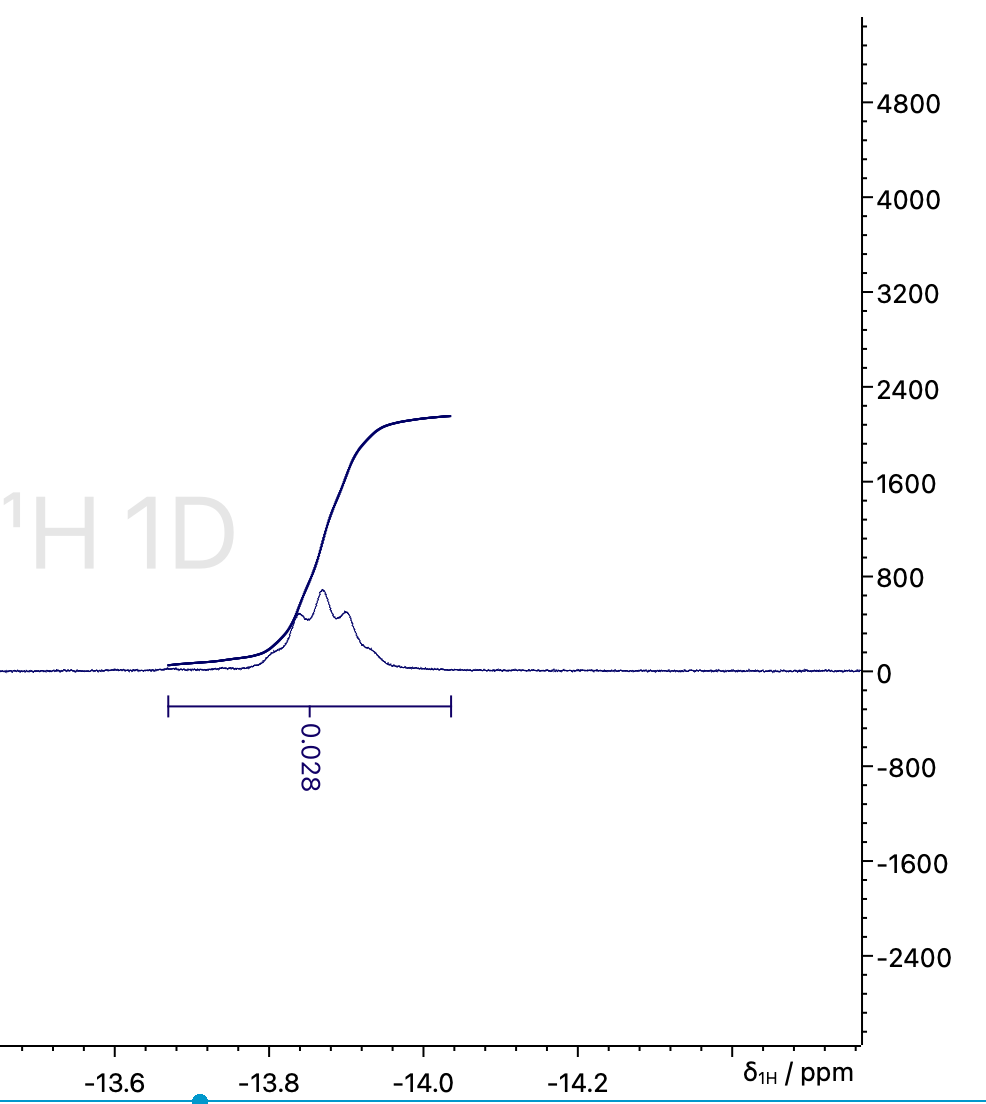
\includegraphics[width=0.8\linewidth]{Relazione/foto/CoH_hydridepeak_right.png}
    \caption{Caption}
    \label{fig:my_label}
\end{figure}




\section{Inserzione di idrogeno in \ce{WO3} e  test di conducibilità}
\subsection{Sintesi}
\subsubsection{Procedura sperimentale}

Abbiamo unito 50 mL di acido cloridrico 3 M ad un becher contenente 0.5 g di triossido di tungsteno e quindi abbiamo aggiunto 1 g di limatura di zinco. Al termine dell’effervescenza abbiamo filtrato su Buchner e raccolto il contenuto in una provetta. Abbiamo ottenuto 0.5123 g di prodotto, ma non essendo il prodotto di stechiometria nota non è possibile calcolare la resa della reazione.




\subsubsection{Commenti e osservazioni}


Il solido prodotto si presentava come sostanza nero antracite con sfumature blu. Il colore che abbiamo ottenuto è sintomo di una reazione ben riuscita; si veda \cite{conduzione}. Il solido si presentava come una dispersione polverosa con particelle molto fini.
\ce{WO3} era molto denso così come la polvere ottenuta. %Peroskiti hanno proprietà di conduttori e semiconduttori.

\subsection{Test conducibilità}

Per caratterizzare il composto sintetizzato abbiamo eseguito due prove di conducibilità elettrica. I dati raccolti sono stati raccolti nella \autoref{tab:conduci} nella \autoref{sec:dati}.







\begin{appendix}
\section{Sistema per il vuoto-azoto}

\section{Dati e tabelle}
\label{sec:dati}
\subsection{Tabelle}
In questa sezioni sono presente tutte le informazioni notate usate per i calcoli\footnote{I dati di densità sono stati presi dall'etichette delle bottiglie o dal sito SigmaAldrich}.
\begin{table}[ht!]
    

\textbf{Densità \hspace{8mm}}
\vspace{1mm}
\begin{tabular}{l c}
\hline Composto & Densità $[\mathrm{g} / \mathrm{mL}]$\\
\hline\hline en & 0.899 \\
\ce{Et2en} & 0.827 \\
$\mathrm{HCOH}$ & 1.09 \\
$\mathrm{CH}_3 \mathrm{NO}_2$ & 1.127 \\
$\mathrm{P}(\mathrm{OPh})_3$ & 1.184 \\
Aldeide Salicilica & 1.146 \\
\hline
\end{tabular}

\end{table}
\begin{table}[ht!]
  \vspace{1mm}  
\textbf{Massa molare}
\begin{tabular}{ l c }
\hline Composto & Massa molare $[\mathrm{g} / \mathrm{mol}]$ \\
\hline\hline 
 \ce{NiCl2}& 129.6 \\

$\mathrm{NiCl}_2 \cdot 6 \mathrm{H}_2 \mathrm{O}$ & 237.70 \\
 $\mathrm{NiBr}_2 \cdot 3 \mathrm{H}_2 \mathrm{O}$ & 272.55 \\
\ce{[Ni(NH3)6]Cl2}& $231.78 $
 \\ $\left[\mathrm{Ni}\left(\mathrm{Et}_2 \mathrm{en}\right)_2\left(\mathrm{H}_2 \mathrm{O}\right)_2\right] \mathrm{Br}_2$ & 486.93 \\
$\left[\mathrm{Ni}\left(\mathrm{Et}_2 \mathrm{en}\right)_2 \mathrm{Br}_2\right]$ & 450.90 \\
 $\mathrm{CoCl}_2 \cdot 6 \mathrm{H}_2 \mathrm{O}$ & 237.93 \\
$\left[\mathrm{Co}(\mathrm{en})_3\right] \mathrm{Cl}_3$ & 345.58 \\
$\left[\mathrm{Ni}(\mathrm{en})_3\right] \mathrm{Cl}_2 \cdot 2 \mathrm{H}_2 \mathrm{O}$ & 345.92 \\
en & 60.10 \\
 $\mathrm{Et}_2 \mathrm{en}$ & 116.20 \\
$[\mathrm{Co}($ dinosar $)] \mathrm{Cl}_3$ & 539.73 \\
$\mathrm{Co}\left(\mathrm{NO}_3\right)_2 \cdot$ \ce{H2O} & 291.03 \\
 $\mathrm{CH}_3 \mathrm{NO}_2$ & 61.04 \\
 $\mathrm{P}(\mathrm{OPh})_3$ & 310.28 \\
 $\mathrm{HCo}\left[\mathrm{P }(\mathrm{OPh})_3\right]_4$ & 1301.02 \\
 
 $\mathrm{HCOH}$ & 30.03 \\

 \ce{WO3}  & 231.84 \\

 \ce{Co(salen)} &  
325.23 \\
 \ce{Cr2(OAc)4 2.H2O } &  788.40 \\
 \ce{K2Cr2O7 } &  294.19 \\
  \ce{Zn } &  	65.41 \\
  Aldeide Salicilica & 	122.12 \\
  \ce{NaBH4} &37.83\\
\hline
\end{tabular}

\end{table}
\subsection{Dati raccolti}


\begin{table}[ht!]
    

\textbf{Provette}
\vspace{1mm}
\begin{tabular}{lcc}
\hline Composto & Massa finale $[\mathrm{g}] $ & Tara $[\mathrm{g}]$ \\
\hline\hline 
$\left[\mathrm{Ni}(\mathrm{en})_3\right] \mathrm{Cl}_2 \cdot 2 \mathrm{H}_2 \mathrm{O}$ & 19.4424  & 15.1714\\
\ce{[Ni(NH3)6]Cl2}& 17.7280 & 15.1515
 \\ $\left[\mathrm{Ni}\left(\mathrm{Et}_2 \mathrm{en}\right)_2\left(\mathrm{H}_2 \mathrm{O}\right)_2\right] \mathrm{Br}_2$ & 17.1101 & 15.0134 
 \\ $\left[\mathrm{Ni}\left(\mathrm{Et}_2 \mathrm{en}\right)_2 \mathrm{Br}_2\right]$ tappo & 21.6770 & 21.6120 \\
$\left[\mathrm{Ni}\left(\mathrm{Et}_2 \mathrm{en}\right)_2 \mathrm{Br}_2\right]$ & 15.8230 & 15.0129  \\

$\left[\mathrm{Co}(\mathrm{en})_3\right] \mathrm{Cl}_3$ $\#1$ & 19.2535 & 15.1411 \\
$\left[\mathrm{Co}(\mathrm{en})_3\right] \mathrm{Cl}_3$ $\#2$ & 18.9275 & 15.1711 \\

$[\mathrm{Co}($ dinosar $)] \mathrm{Cl}_3$ & 17.7611 & 15.0861 \\ $\mathrm{HCo}\left[\mathrm{P }(\mathrm{OPh})_3\right]_4$ & 15.6794 & 15.0190 \\
 \ce{Co(salen)} & 18.8692 & 15.1226\\
 \ce{[Cr2(OAc)4].2H2O } & 17.6259 & 15.0654\\
 
\hline
\end{tabular}

\end{table}


\begin{table}[ht!]
\textbf{Misure magnetiche}
\vspace{1mm}
\begin{tabular}{lccc}
 \hline 
 Composto & Altezza [cm] & Massa$[\mathrm{g}] $ & Misura   \\
\hline\hline 
 \multirow{4}{*}{$\left[\mathrm{Ni}\left(\mathrm{Et}_2 \mathrm{en}\right)_2\left(\mathrm{H}_2 \mathrm{O}\right)_2\right] \mathrm{Br}_2$} & 3.0 & 1.7547 & 93\\ 

& 3.4 & 1.7714 & 109 \\
& 2.6 & 1.7529 & 108 \\
& 2.9 & 1.7598 & 110 \\

\hline
 \multirow{4}{*}{ \ce{[Ni(en)3]Cl2}} & 2.7 & 1.7426 & 98 \\ 
 & 3.2 & 1,7515 & 98 \\
& 3.4 & 1,7551 & 99 \\
& 2.7 & 1.7423 & 97 \\


 
\hline
\end{tabular}

\caption{La massa della provetta utilizza è 1.6929 g, mentre il valore fornito dallo strumento per la provetta vuota è -65.}
\label{tab:magnet}
\end{table}
\begin{table}[ht!]
\textbf{Pesate}
\vspace{1mm}
\begin{tabular}{lc}
\hline Composto & Massa finale $[\mathrm{g}] $ \\
\hline\hline 
 $\left[\mathrm{Ni}\left(\mathrm{Et}_2 \mathrm{en}\right)_2\left(\mathrm{H}_2 \mathrm{O}\right)_2\right] \mathrm{Br}_2$ & 0.8751\\ 

 \ce{[Co(en)3]Cl3} & 2.450 \\
 
 
\ce{[Ni(NH3)6]Cl2}  & 
1.1532\\
 \ce{[Ni(en)3]Cl2.2H2O}& 1.7250\\
   \ce{[Ni(Eten)22H2O]Br2}&0.4521\\
\hline
\end{tabular}
\label{tab:pesate}
\end{table}


\begin{table}[ht!]
    \textbf{Misure di conducibilità}
    \begin{tabular}{l c c }
   Composto  & Massa[g] & Resistenza[$\Omega$] \\
   \hline\hline
       \ce{H_xWO3}  &  0.247 & 2.1 \\
        \ce{H_xWO3} trattato & 0.233  & $9 \cdot 10^5$\\
        \hline
    \end{tabular}
    \caption{Risultati prove di conducibilità}
    \label{tab:conduci}
\end{table}





\section{Spettri completi}

\begin{figure}
    \centering
    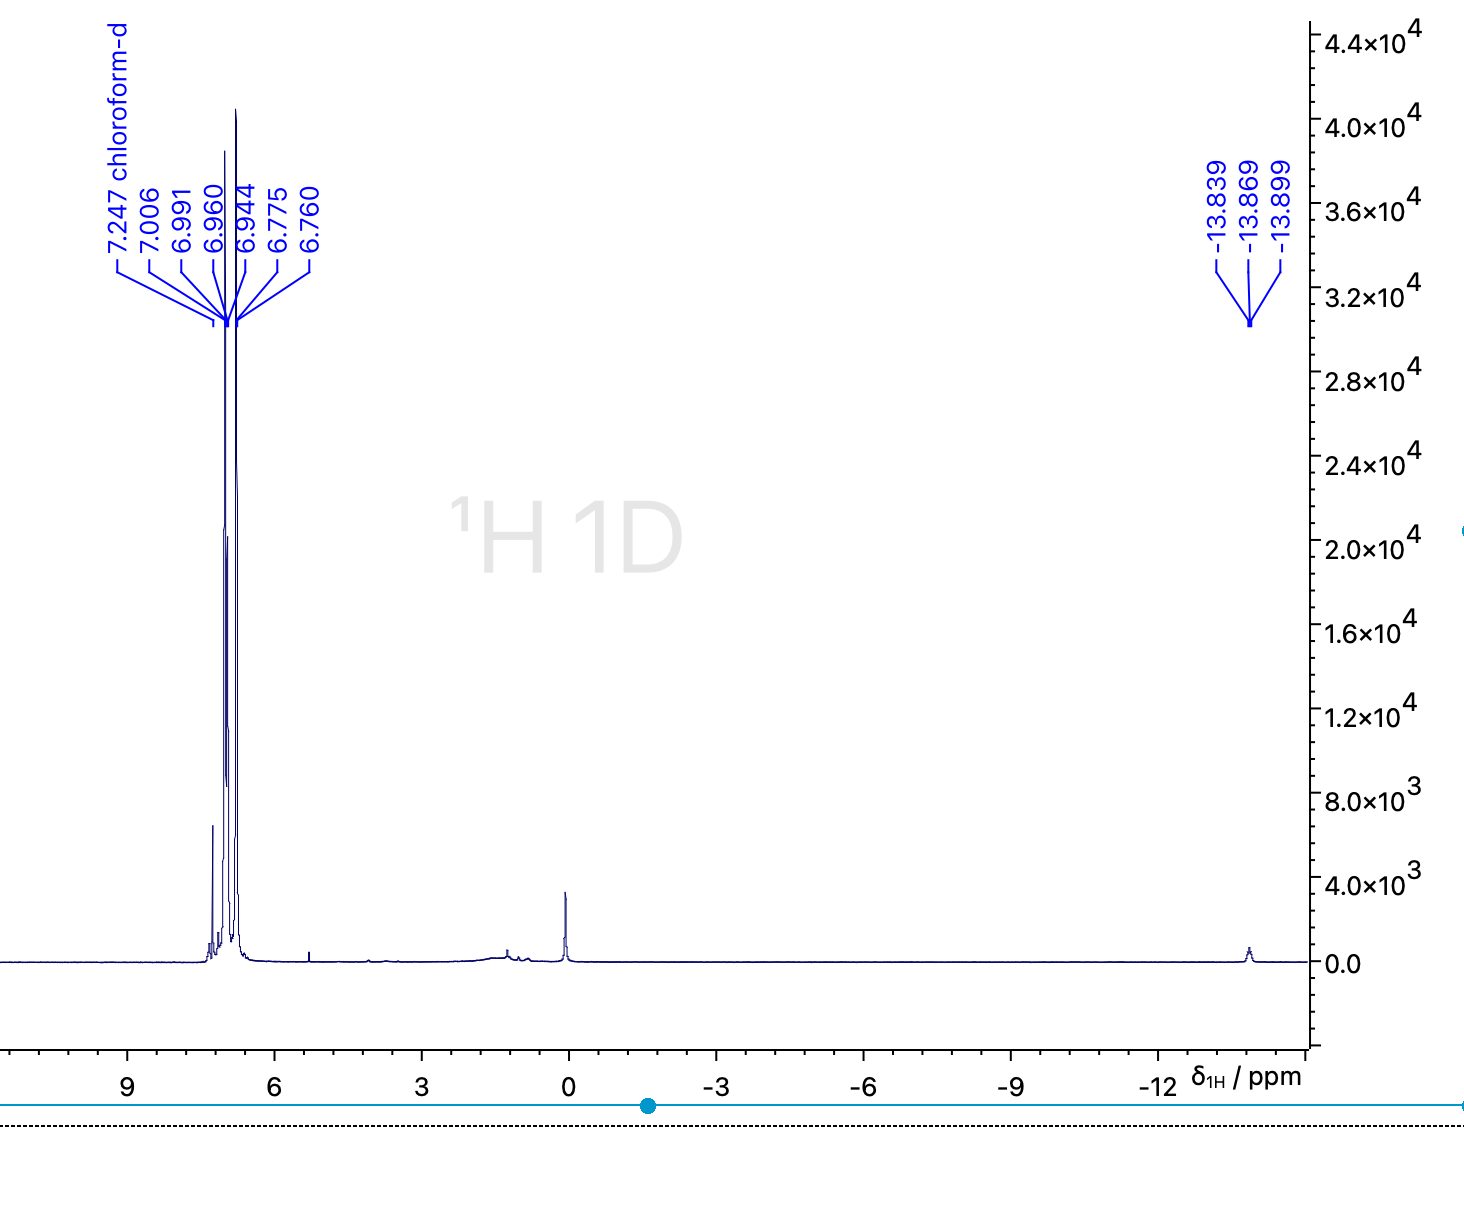
\includegraphics[width=\linewidth]{Relazione/foto/CoH_peak_calcall.png}
    \caption{Caption}
    \label{fig:cohfull}
\end{figure}


\begin{figure}
    \centering
    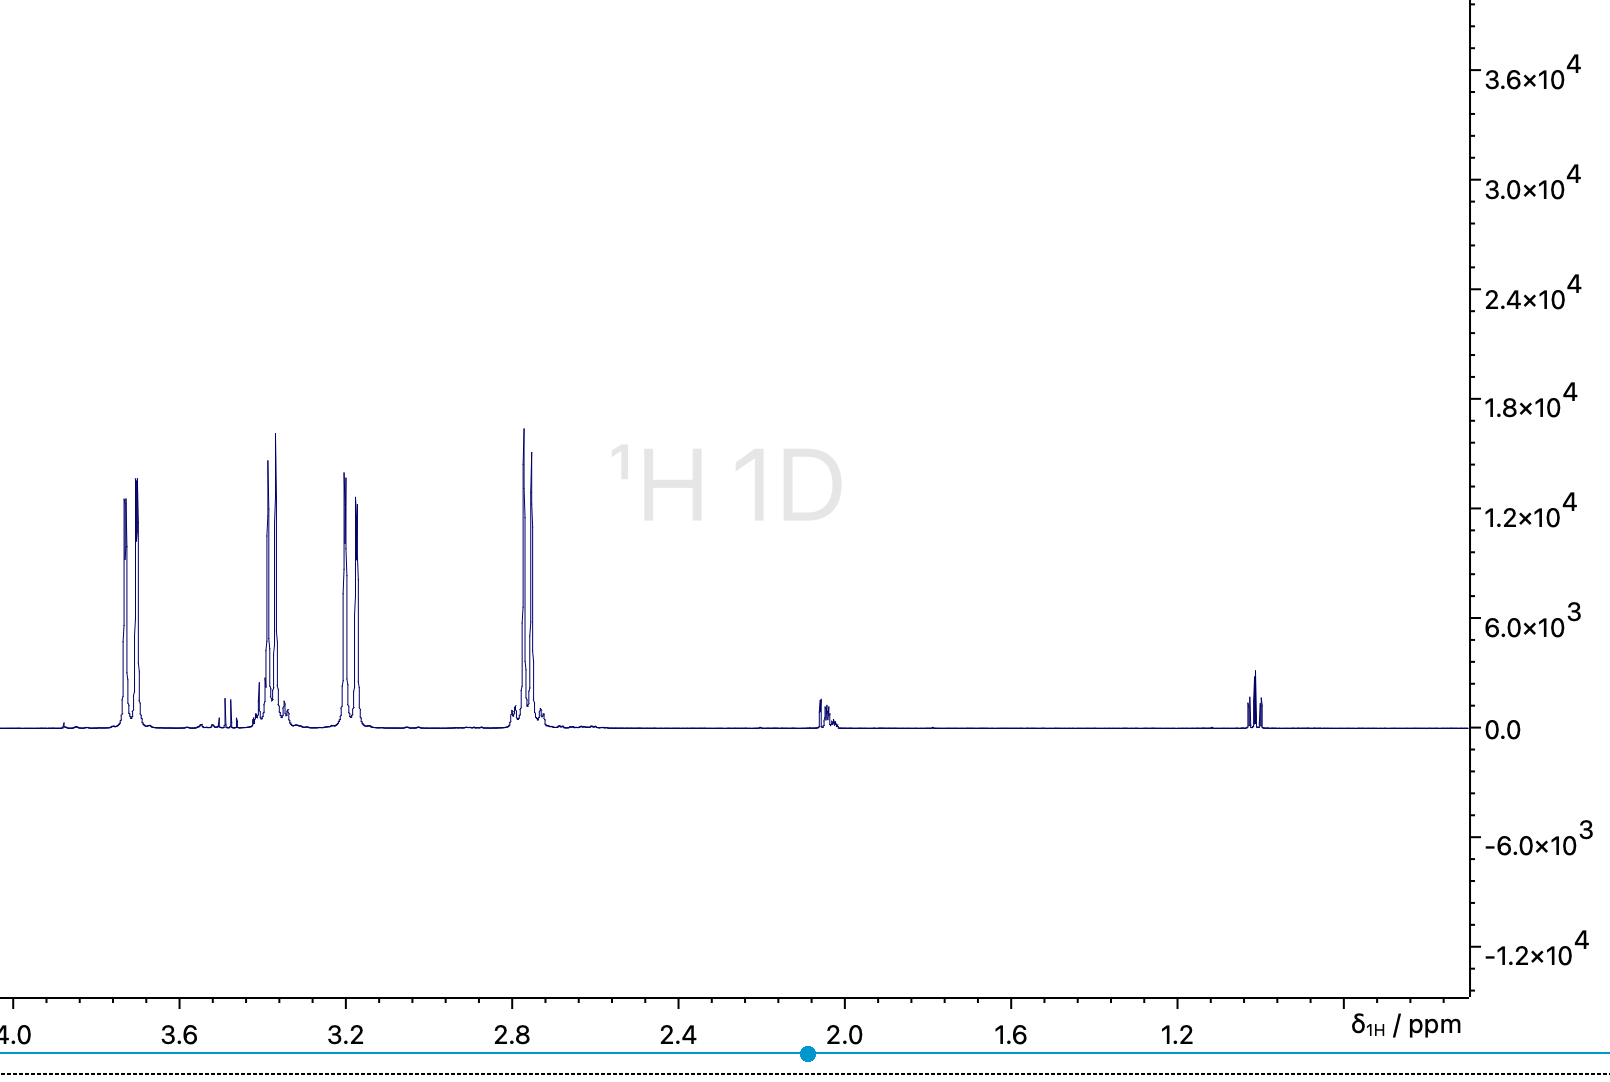
\includegraphics[width=\linewidth]{Relazione/foto/Dinosar_full.png}
    \caption{Caption}
    \label{fig:cohfull}
\end{figure}





\end{appendix}




\clearpage
\printbibliography
\end{document}
